\chapter{Simulation Results}
\label{sec:simulation_results}

All the designs presented in \Cref{sec:comparison} are tested in simulation.
As explained in \Cref{sec:method}, they are simulated in
Gazebo$^\textrm{\textregistered}$ and controlled by the means of a ROS node.
These simulations are performed to evaluate the feasibility and  the controllability
of the theoretical optimal designs obtained in \Cref{sec:optimization_results}.
Furthermore, they also allow for comparison between different MAVs morphologies.\\
The most interesting simulation results obtained are presented in this section.
First, a flight test performed by the tri-copter depicted in \Cref{fig:comp_tri} is
presented, then a comparison between the hexa-copter shown in \Cref{fig:comp_hexa}
and the Voliro from \citep{kamel_voliro:_2018} is proposed. Finally, a manipulation
example with the hepta-copter presented in \Cref{sec:hepta_copter} is shown.

\section{Tri-copter}
\label{sec:tri_copter_sim}

The tri-copter with tilting rotor is a very interesting case because it is holonomic,
which means that it has exactly six degrees of freedom (DoF) and evolves in a
three dimensional space. Therefore, it should theoretically be able to produce forces
and torques in any direction. To verify that a test flight is performed where the MAV
hover at one meter over the ground and changes its orientation up to a pitch angle
$\theta$ equal to $90^{\circ}$. The results of this test can be observed in
\Cref{fig:tri_sim} and it is clear from this quarter pitch flip that the tri-copter
is indeed able to hover in any orientation. It is very thrilling to see that the adapted
control node described in \Cref{sec:control_approach} is truly able to control this
model.

\begin{figure}[!ht]
  \begin{center}
  \begin{minipage}[t]{0.24\textwidth}
    \centering
    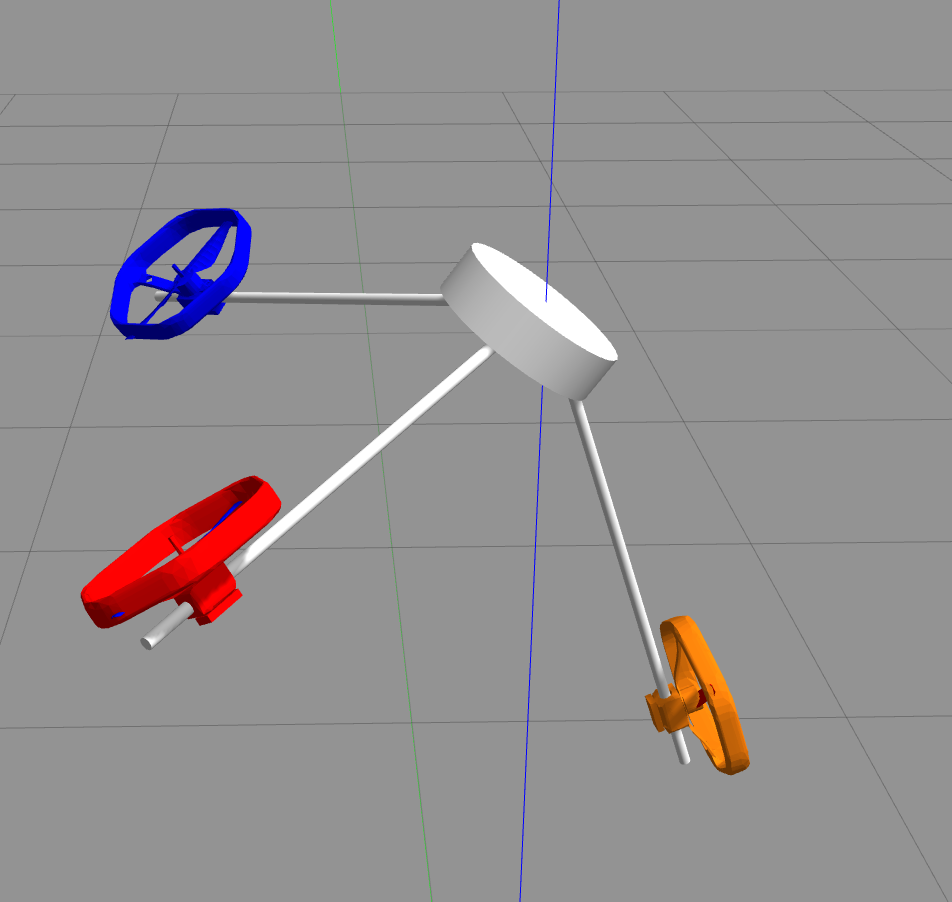
\includegraphics[width=\linewidth]{images/tri_sim1.png}
  \end{minipage}
  \hfill
  \begin{minipage}[t]{0.24\textwidth}
    \centering
    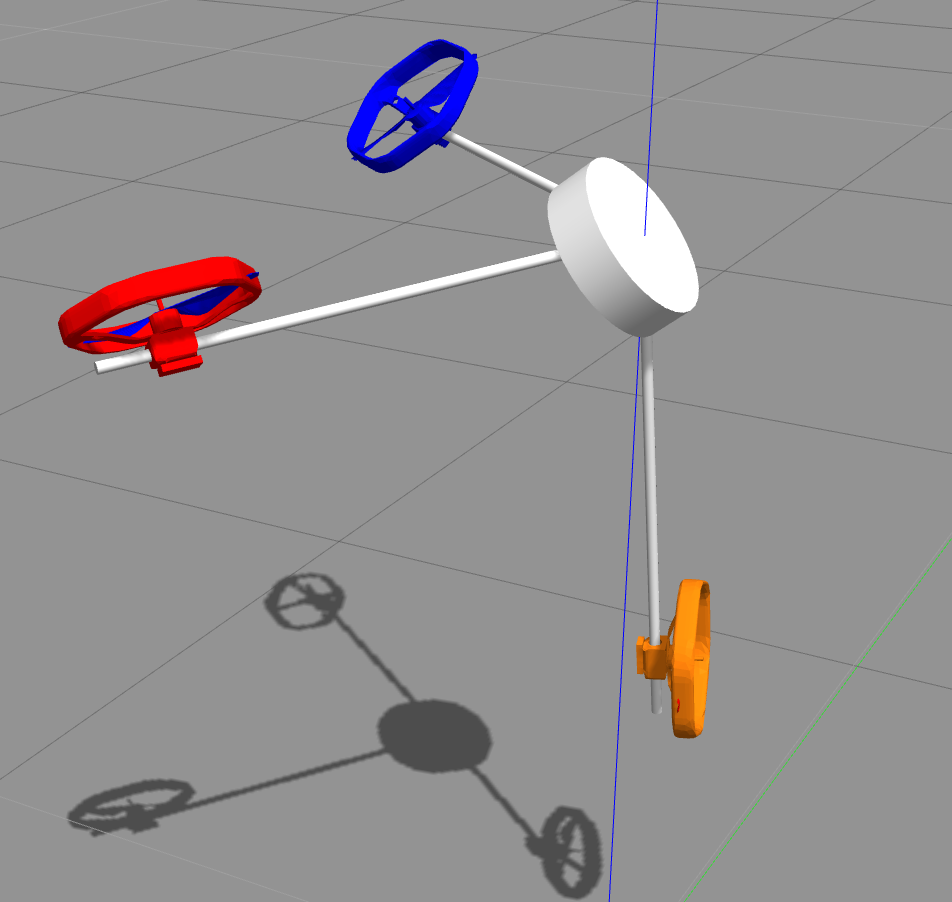
\includegraphics[width=\linewidth]{images/tri_sim2.png}
  \end{minipage}
  \hfill
  \begin{minipage}[t]{0.24\textwidth}
    \centering
    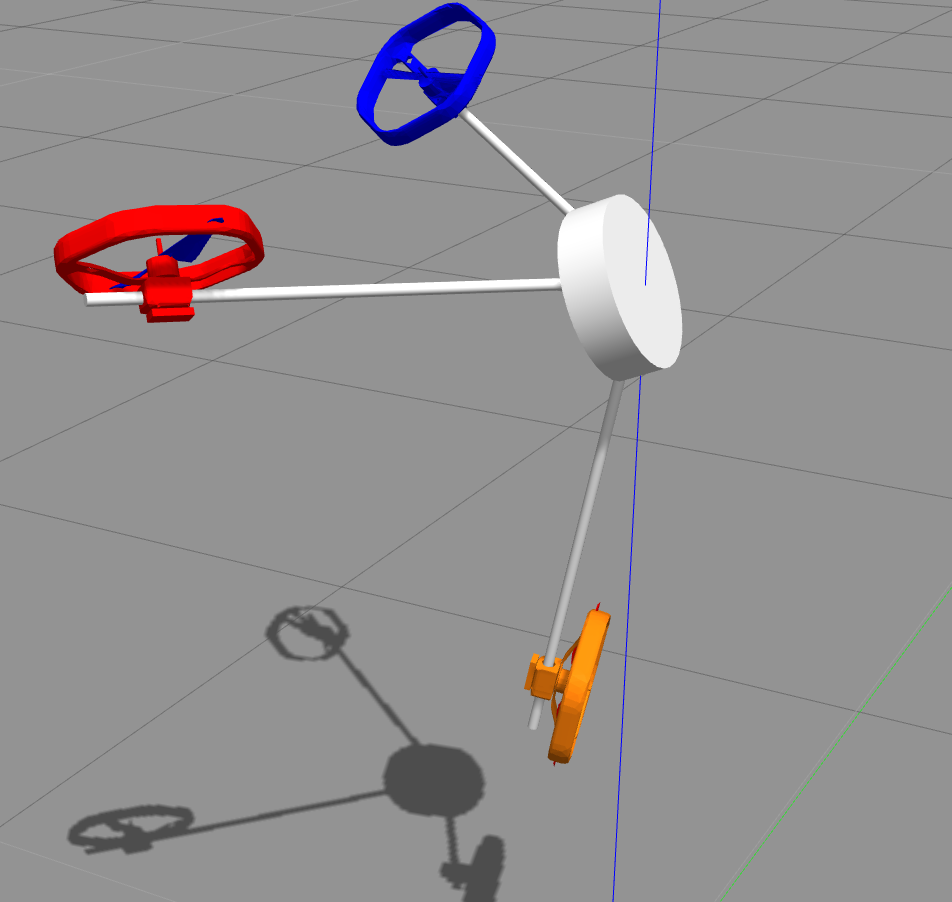
\includegraphics[width=\linewidth]{images/tri_sim3.png}
  \end{minipage}
  \hfill
  \begin{minipage}[t]{0.24\textwidth}
    \centering
    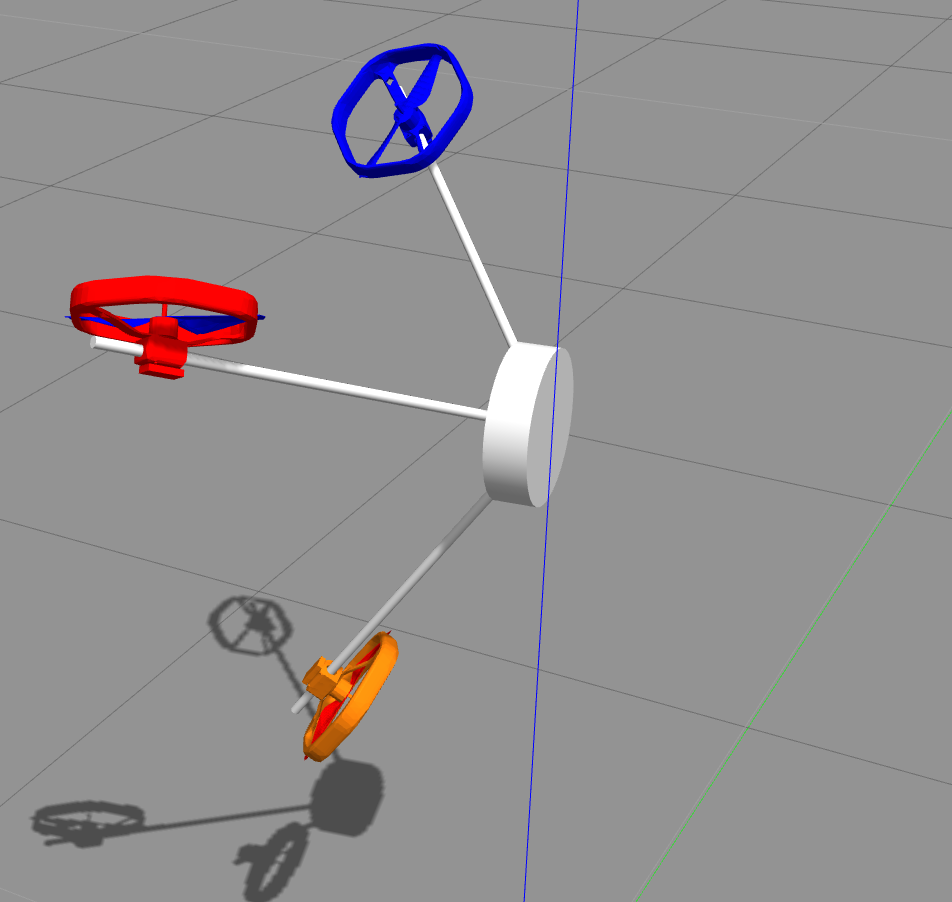
\includegraphics[width=\linewidth]{images/tri_sim4.png}
  \end{minipage}
  \caption{Simulation of the tri-copter in Gazebo.}
  \label{fig:tri_sim}
  \end{center}
\end{figure}

\section{Hexa-copter}
\label{sec:hexa_copter_sim}

\begin{figure}[!ht]
  \resizebox{\textwidth}{!}{\begin{subfigure}[b]{0.5\textwidth}
    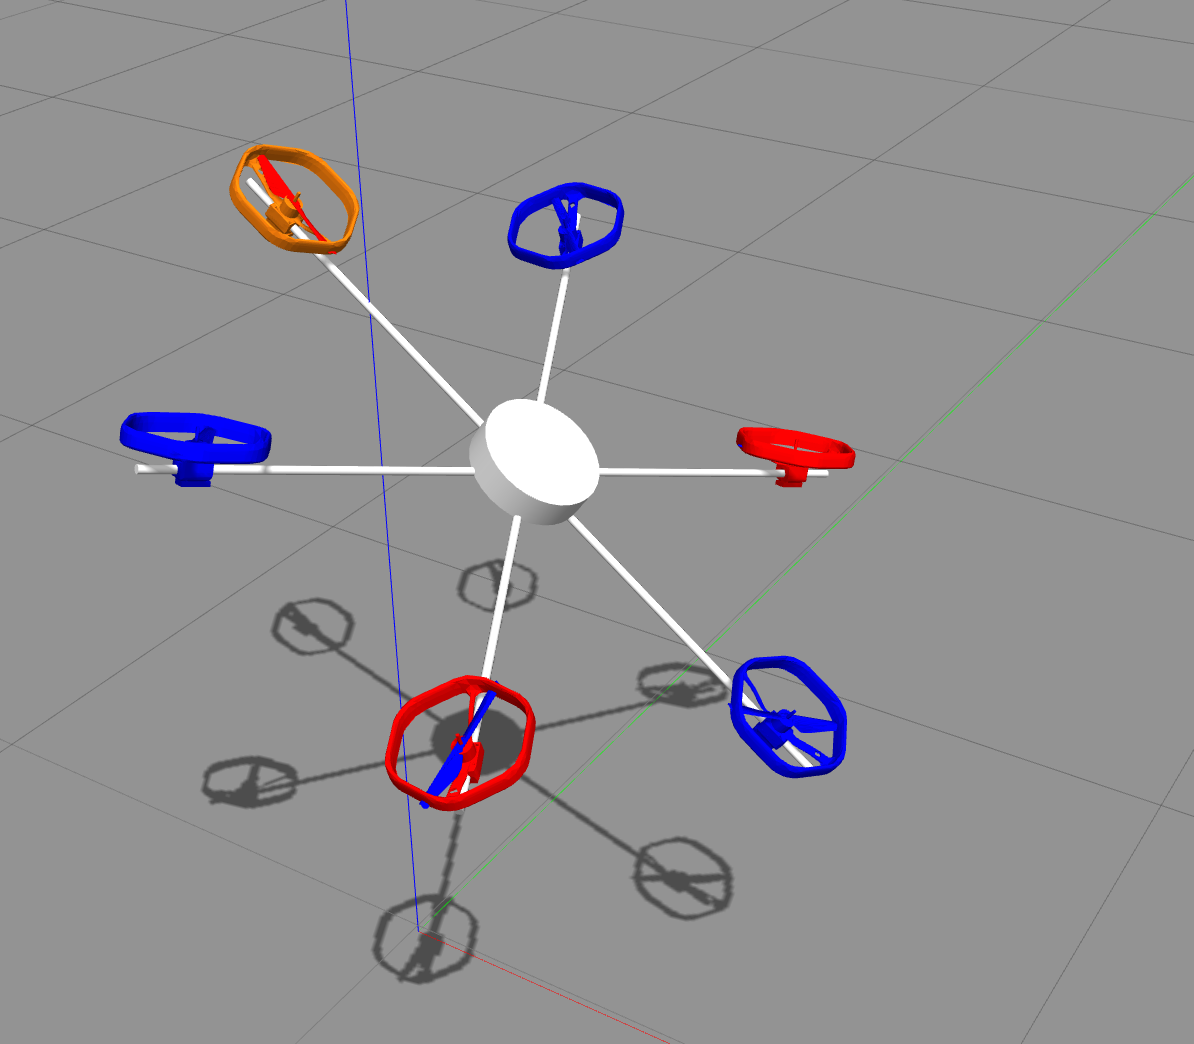
\includegraphics[width=\linewidth]{images/Voliro_sim.png}
    \caption{Voliro.} \label{fig:Voliro_sim}
  \end{subfigure}
  \hspace*{\fill} % separation between the subfigures
  \begin{subfigure}[b]{0.5\textwidth}
    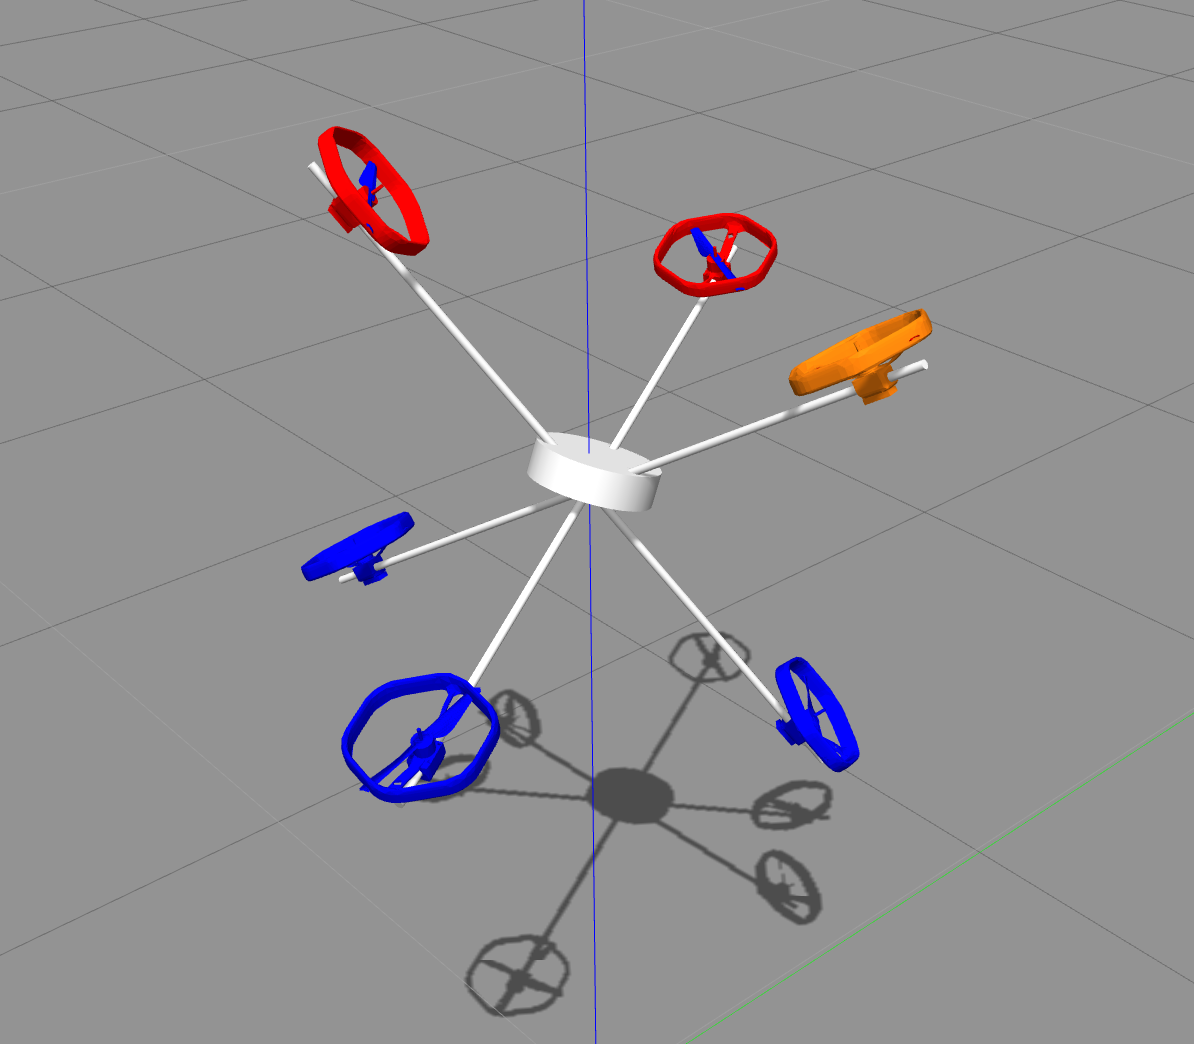
\includegraphics[width=\linewidth]{images/Hexa_sim.png}
    \caption{Optimal hexa-copter.} \label{fig:Hexa_sim}
  \end{subfigure}}
  \caption{Representation of two six-rotors MAV model spawned in Gazebo$^\textrm{\textregistered}$}
  \label{fig:Sim_six_rotors}
\end{figure}

\begin{figure}[!ht]
  \begin{center}
    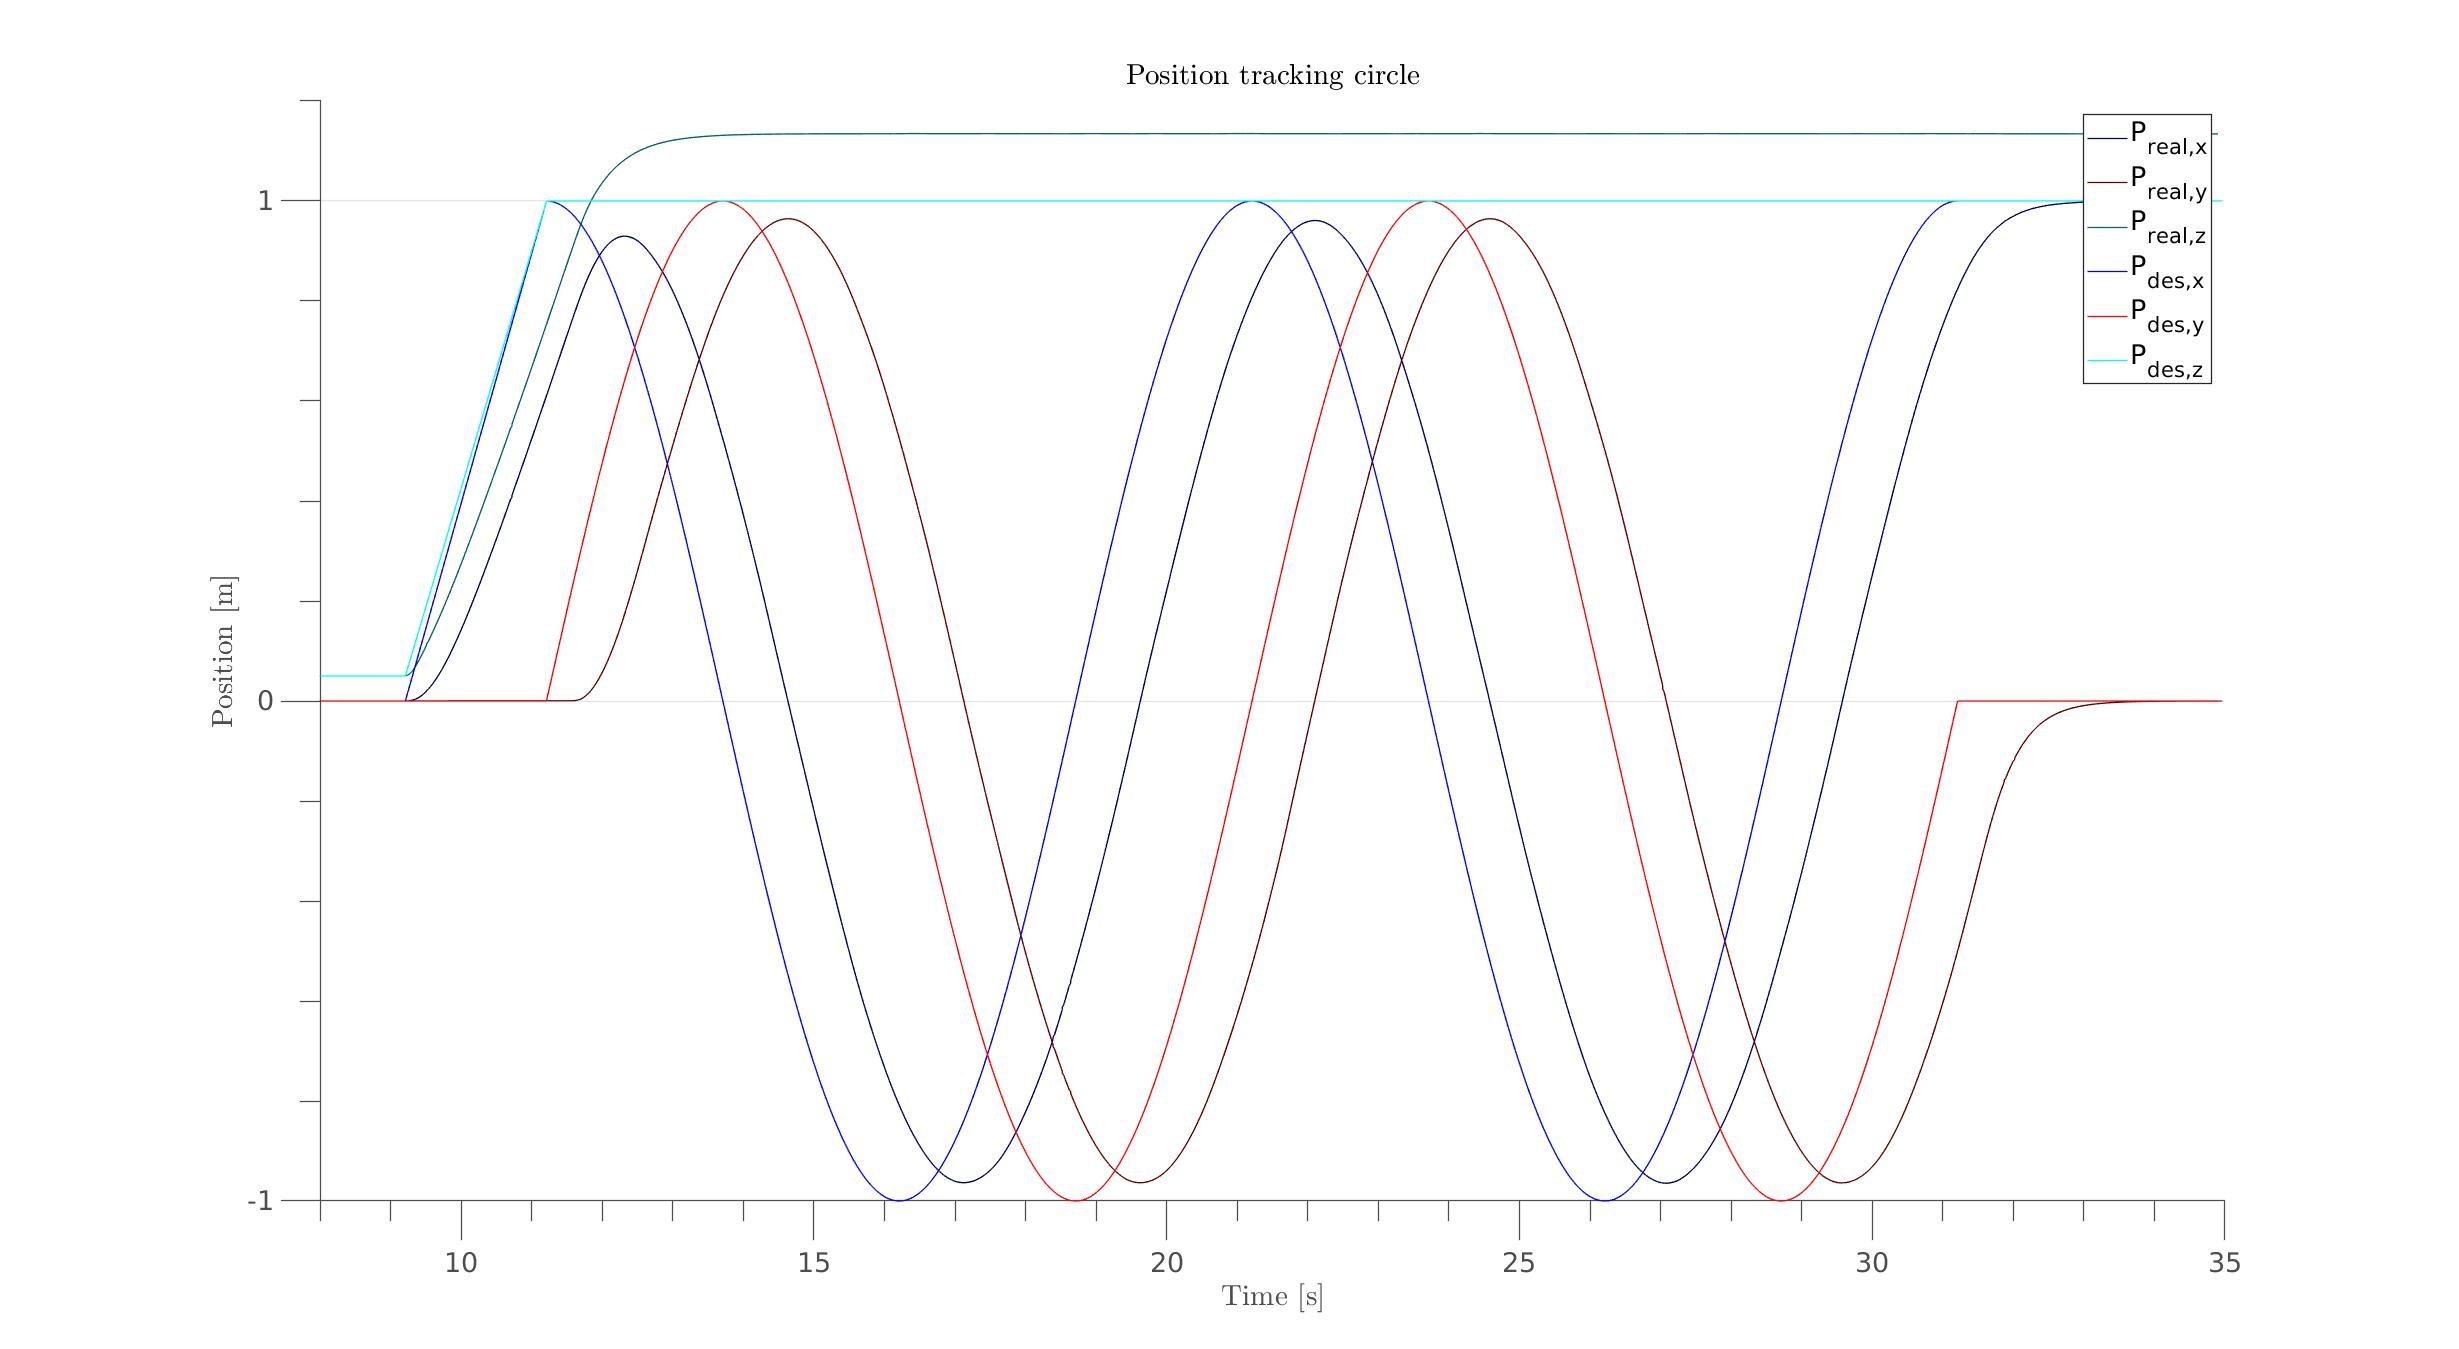
\includegraphics[width=1.0\linewidth]{images/Voliro_circle_position.jpg}
    \caption{Position tracking of a one meter circle performed by Voliro.}
    \label{fig:Voliro_position_circle}
  \end{center}
\end{figure}

\begin{figure}[!ht]
  \begin{center}
    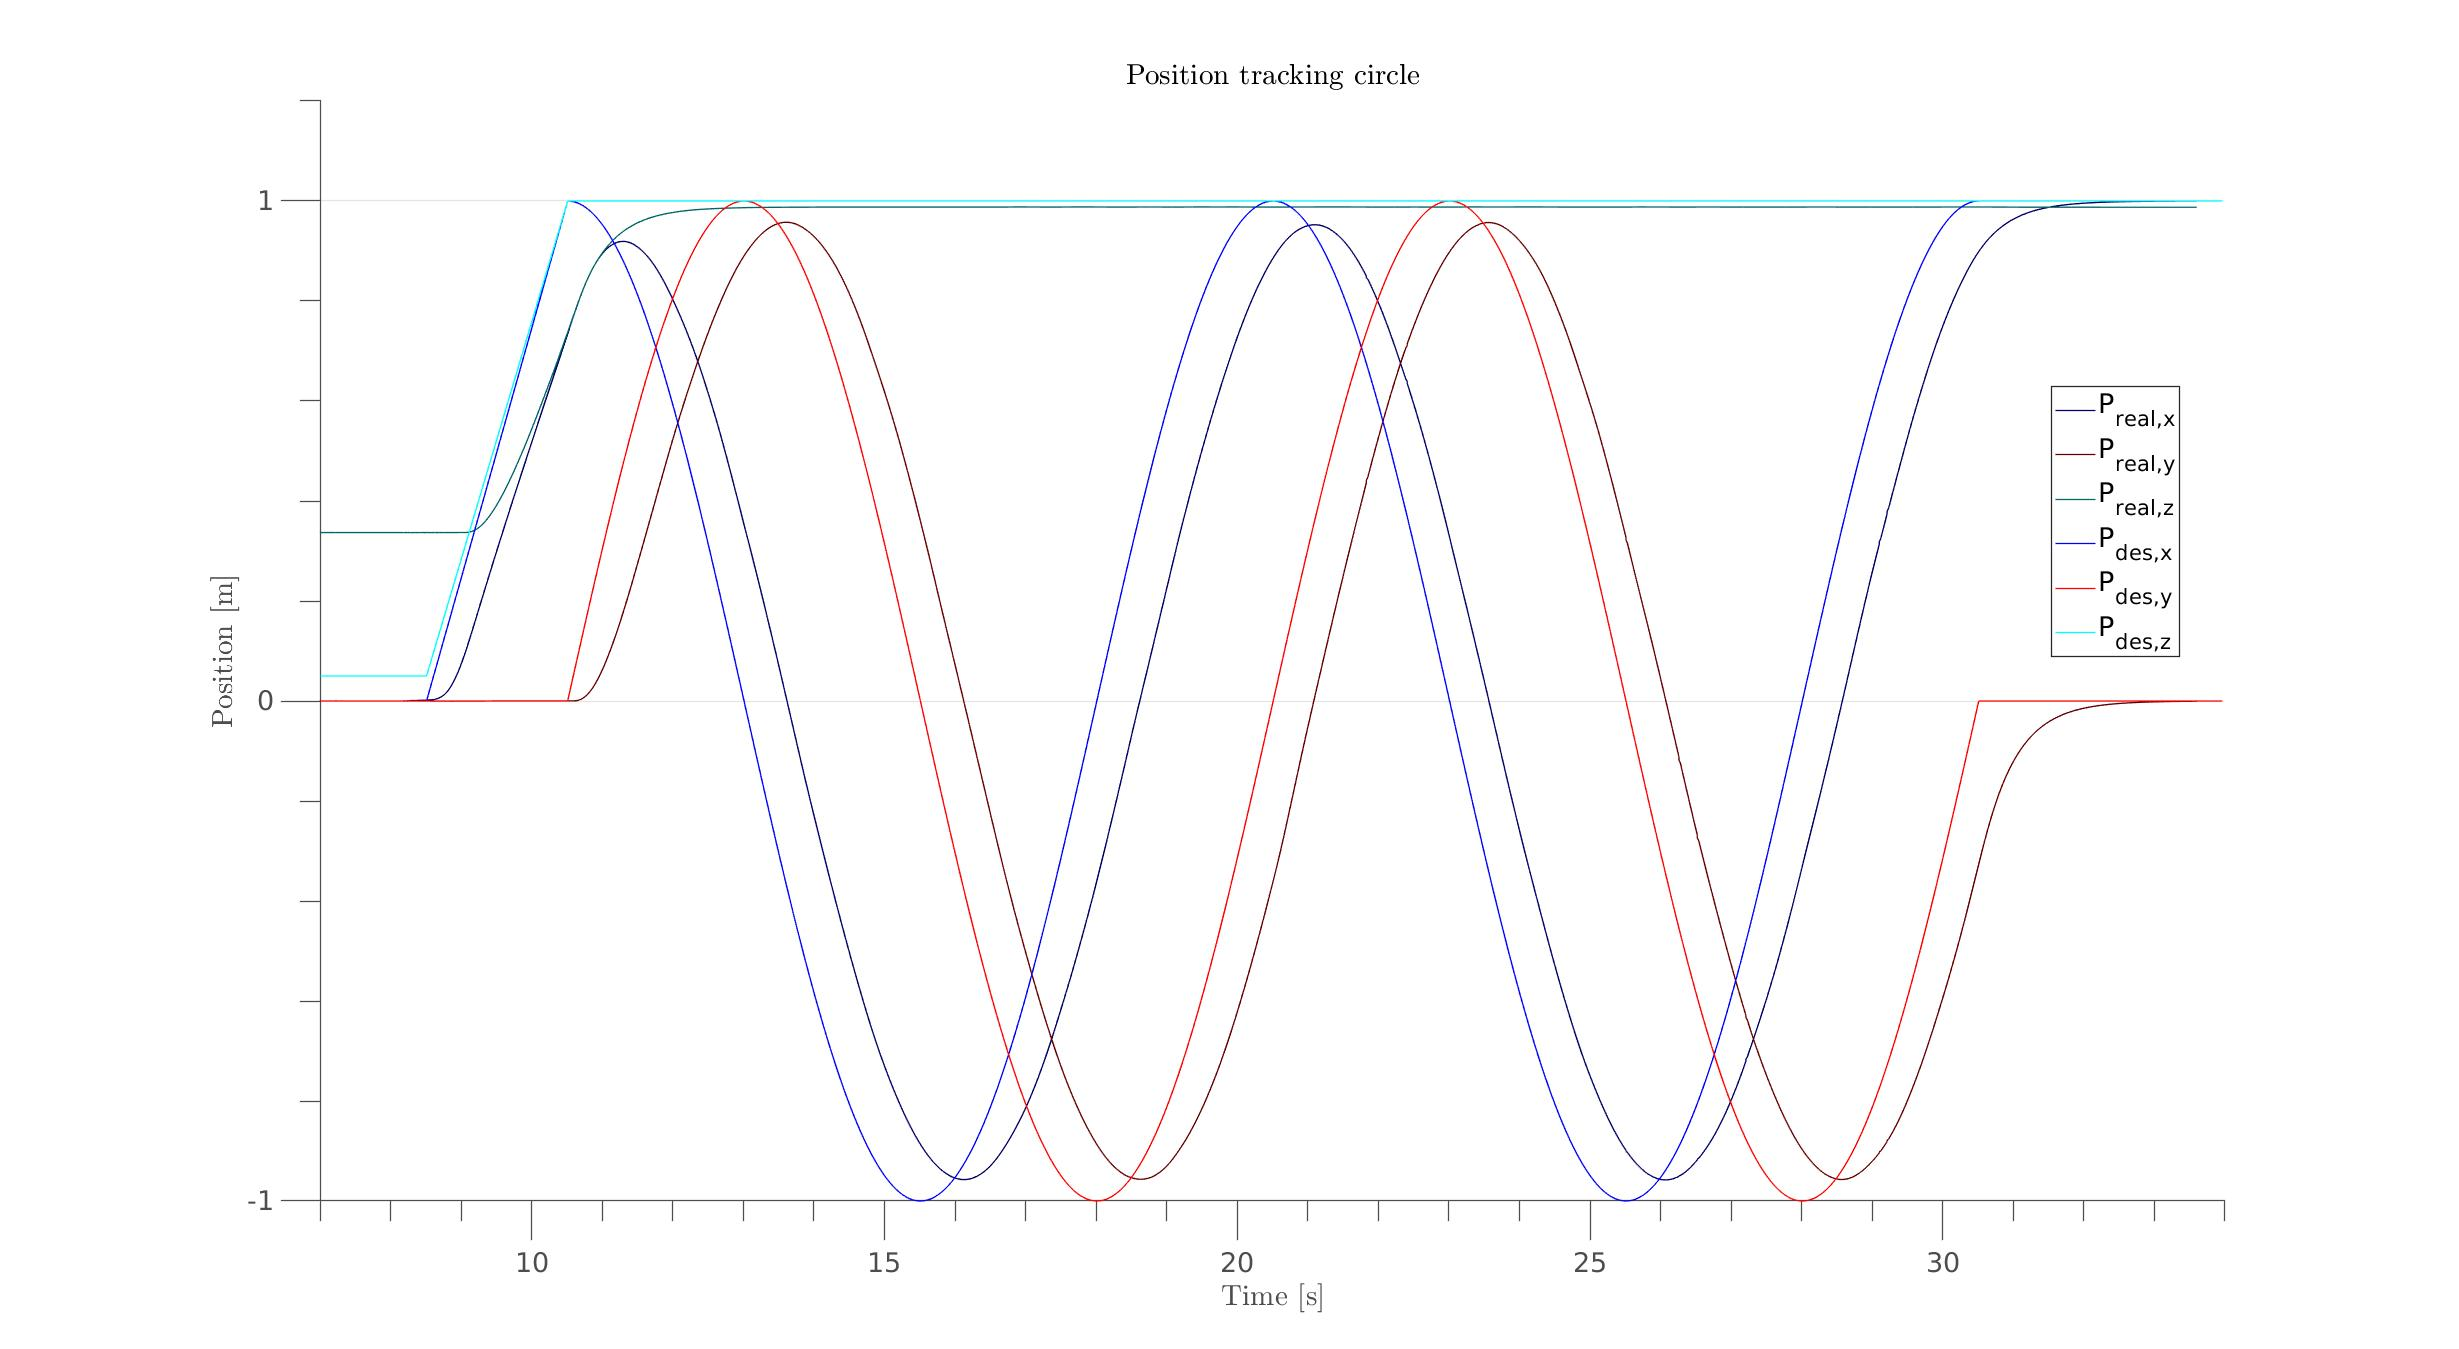
\includegraphics[width=1.0\linewidth]{images/Hexa_circle_position.jpg}
    \caption{Position tracking of a one meter circle performed by the optimal hexa-copter.}
    \label{fig:Hexa_position_circle}
  \end{center}
\end{figure}

\begin{figure}[!ht]
  \begin{center}
    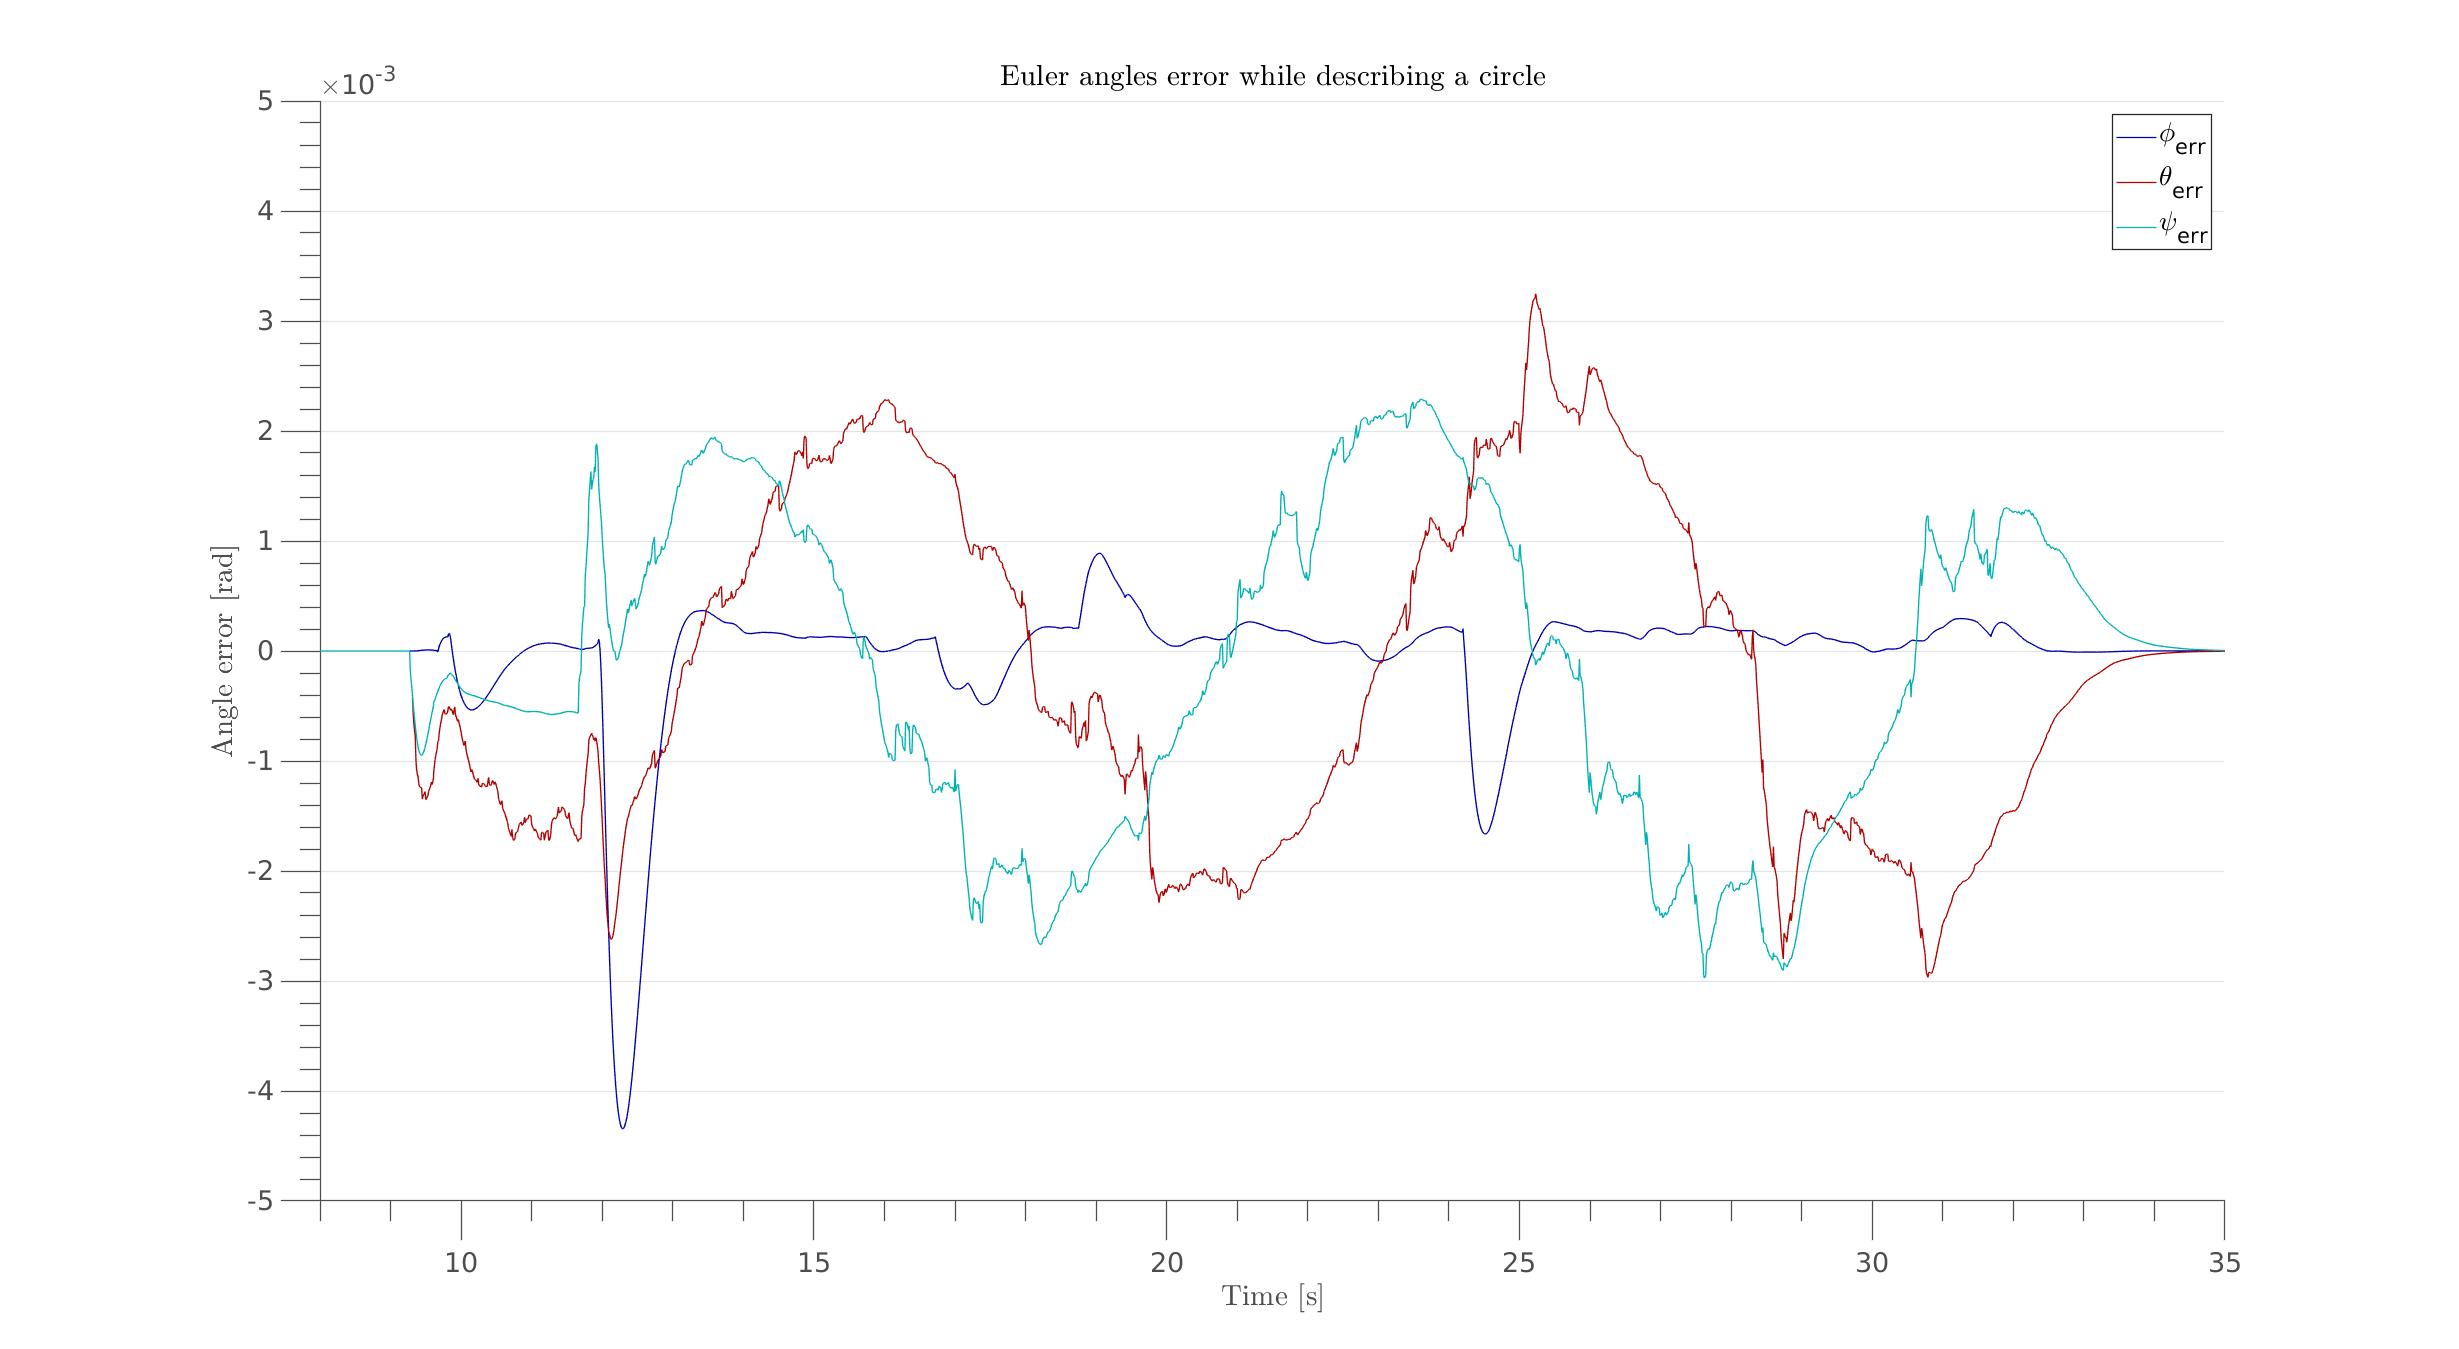
\includegraphics[width=1.0\linewidth]{images/Voliro_circle_angle.jpg}
    \caption{Pitch, roll and yaw angle errors when Voliro track a one meter circle.}
    \label{fig:Voliro_angle_circle}
  \end{center}
\end{figure}

\begin{figure}[!ht]
  \begin{center}
    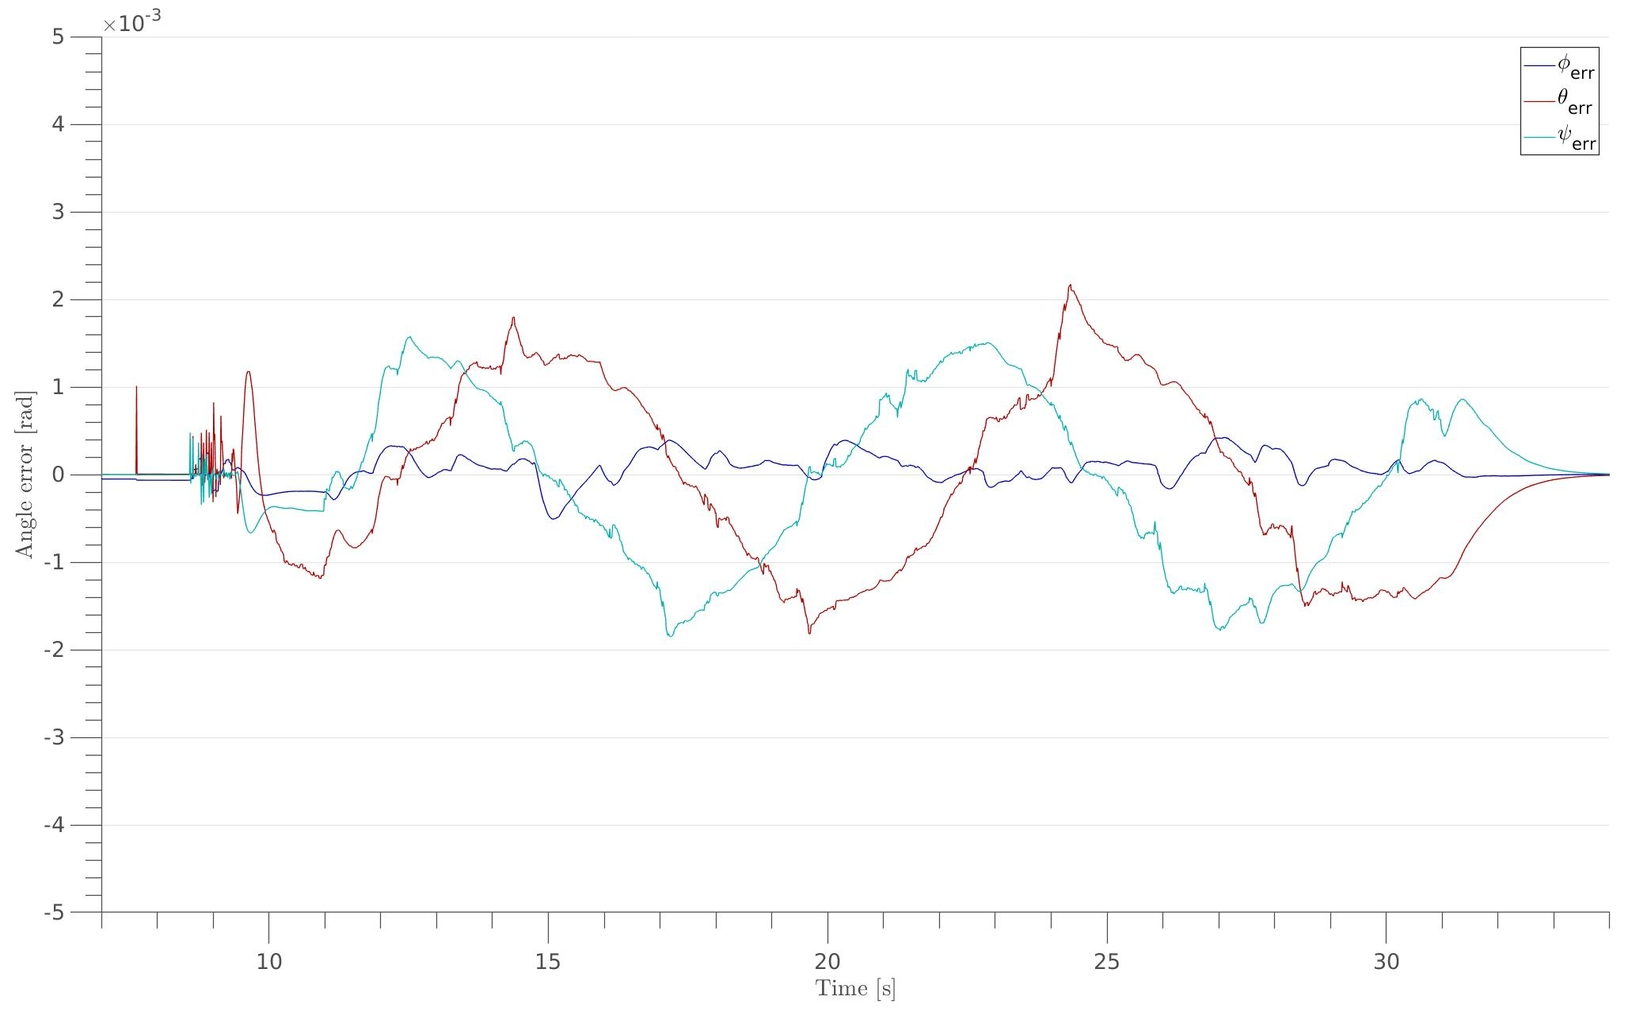
\includegraphics[width=1.0\linewidth]{images/Hexa_circle_angle.jpg}
    \caption{Pitch, roll and yaw angle errors when the optimal hexa-copter track a one meter circle.}
    \label{fig:Hexa_angle_circle}
  \end{center}
\end{figure}

\begin{figure}[!ht]
  \begin{center}
    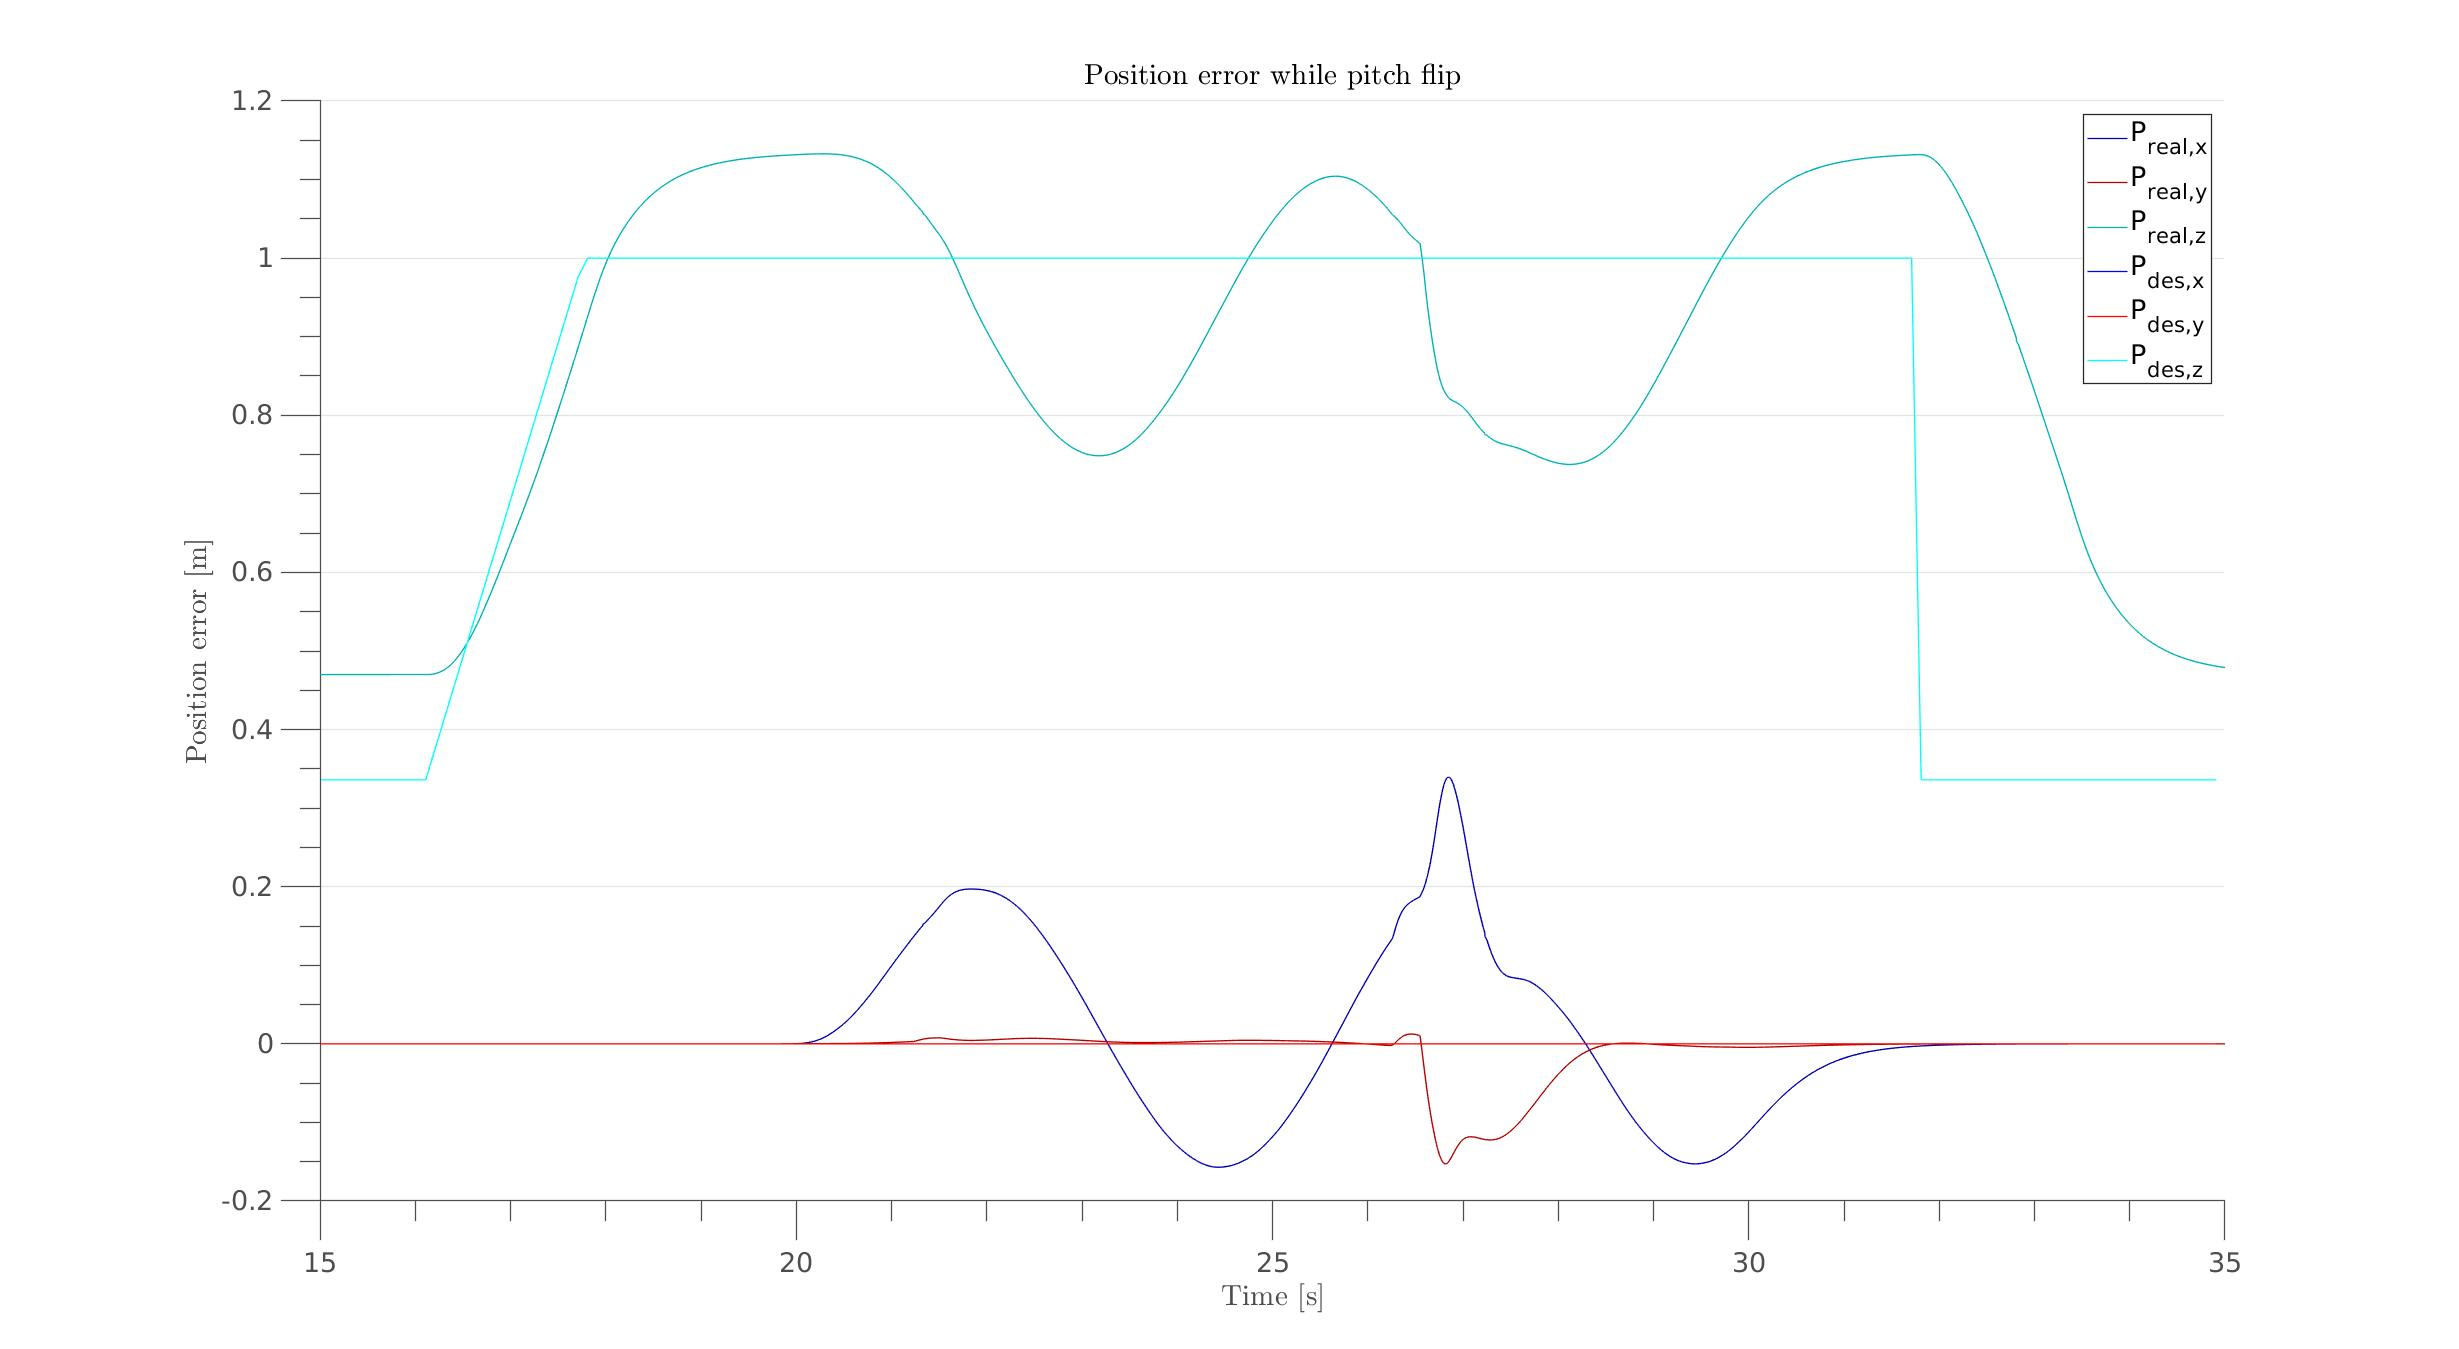
\includegraphics[width=1.0\linewidth]{images/Voliro_pitch_position.jpg}
    \caption{Position tracking for Voliro performing a full pitch flip.}
    \label{fig:Voliro_position_pitch}
  \end{center}
\end{figure}

\begin{figure}[!ht]
  \begin{center}
    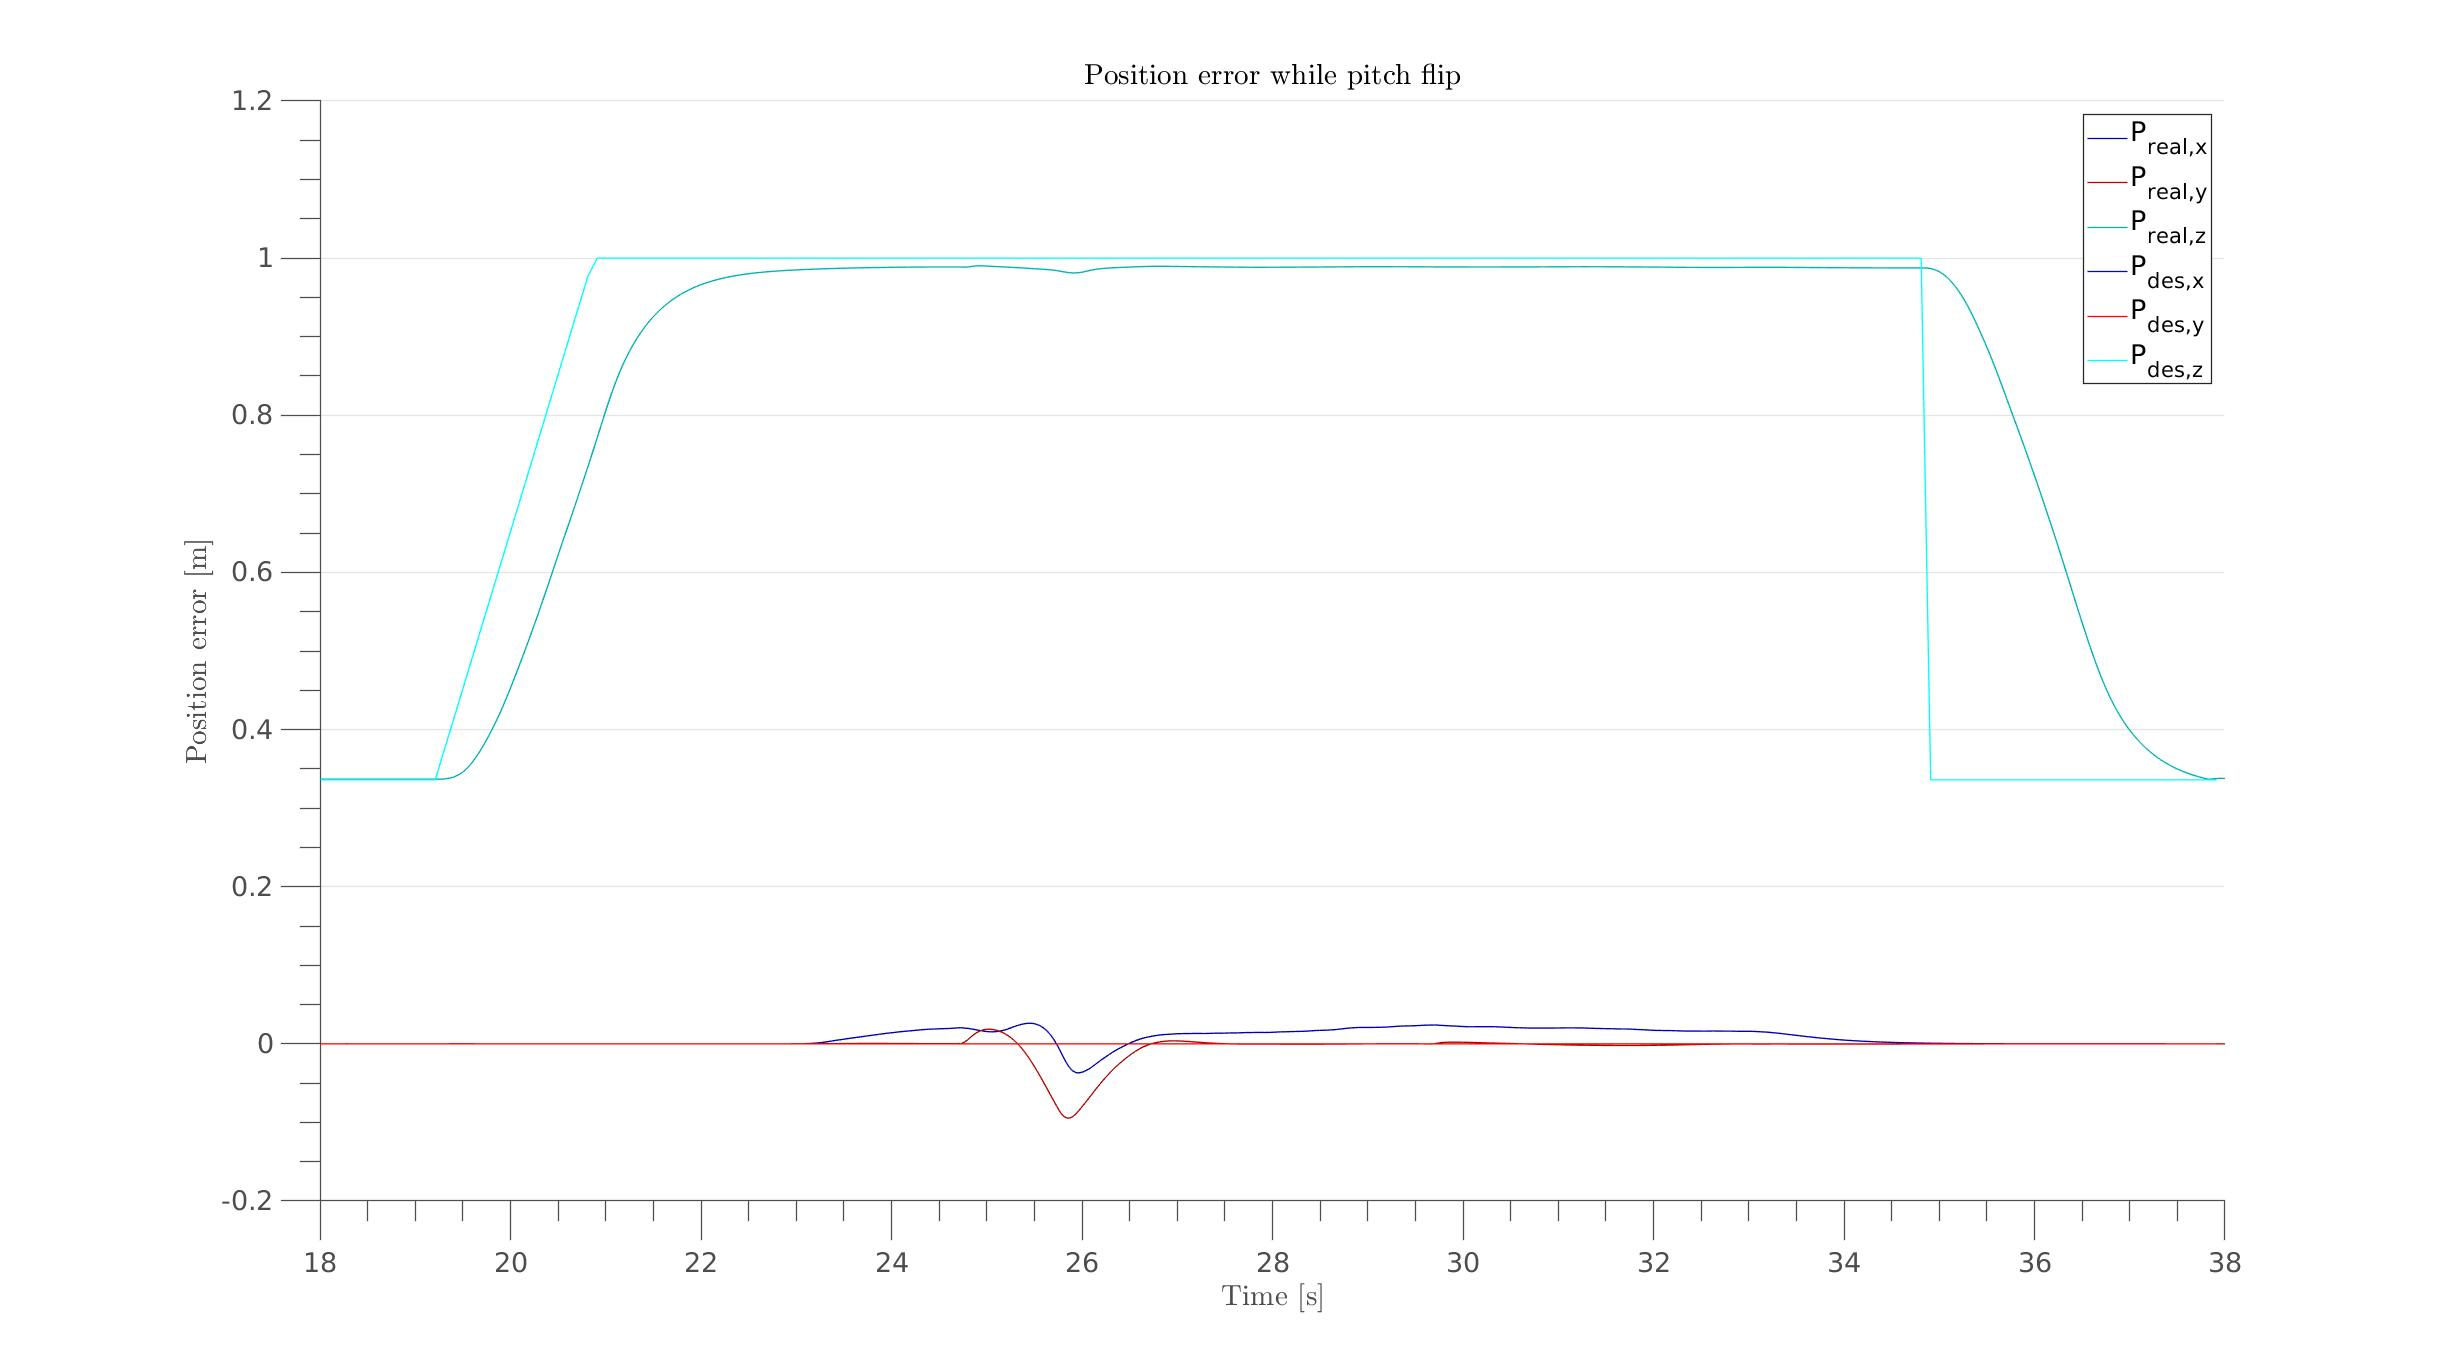
\includegraphics[width=1.0\linewidth]{images/Hexa_pitch_position.jpg}
    \caption{Position tracking for the optimal hexa-copter performing a full pitch flip.}
    \label{fig:Hexa_position_pitch}
  \end{center}
\end{figure}

\begin{figure}[!ht]
  \begin{center}
    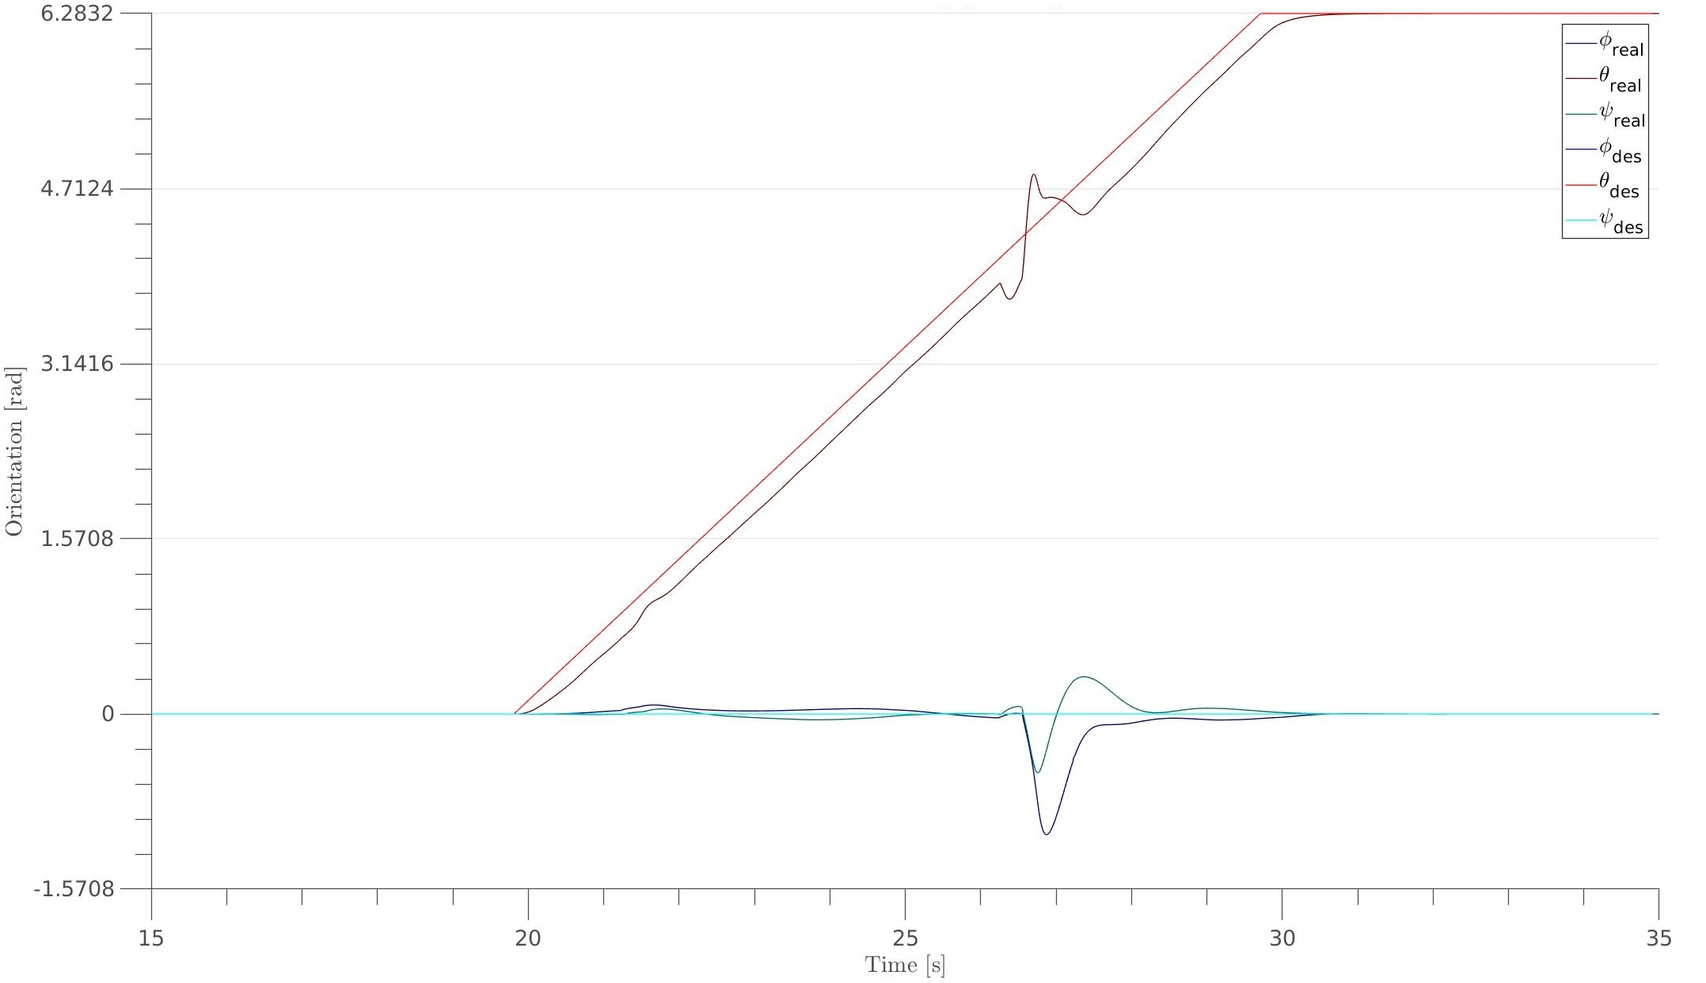
\includegraphics[width=1.0\linewidth]{images/Voliro_pitch_angle.jpg}
    \caption{Pitch, roll and yaw angle tracking for Voliro performing a full pitch flip.}
    \label{fig:Voliro_angle_pitch}
  \end{center}
\end{figure}

\begin{figure}[!ht]
  \begin{center}
    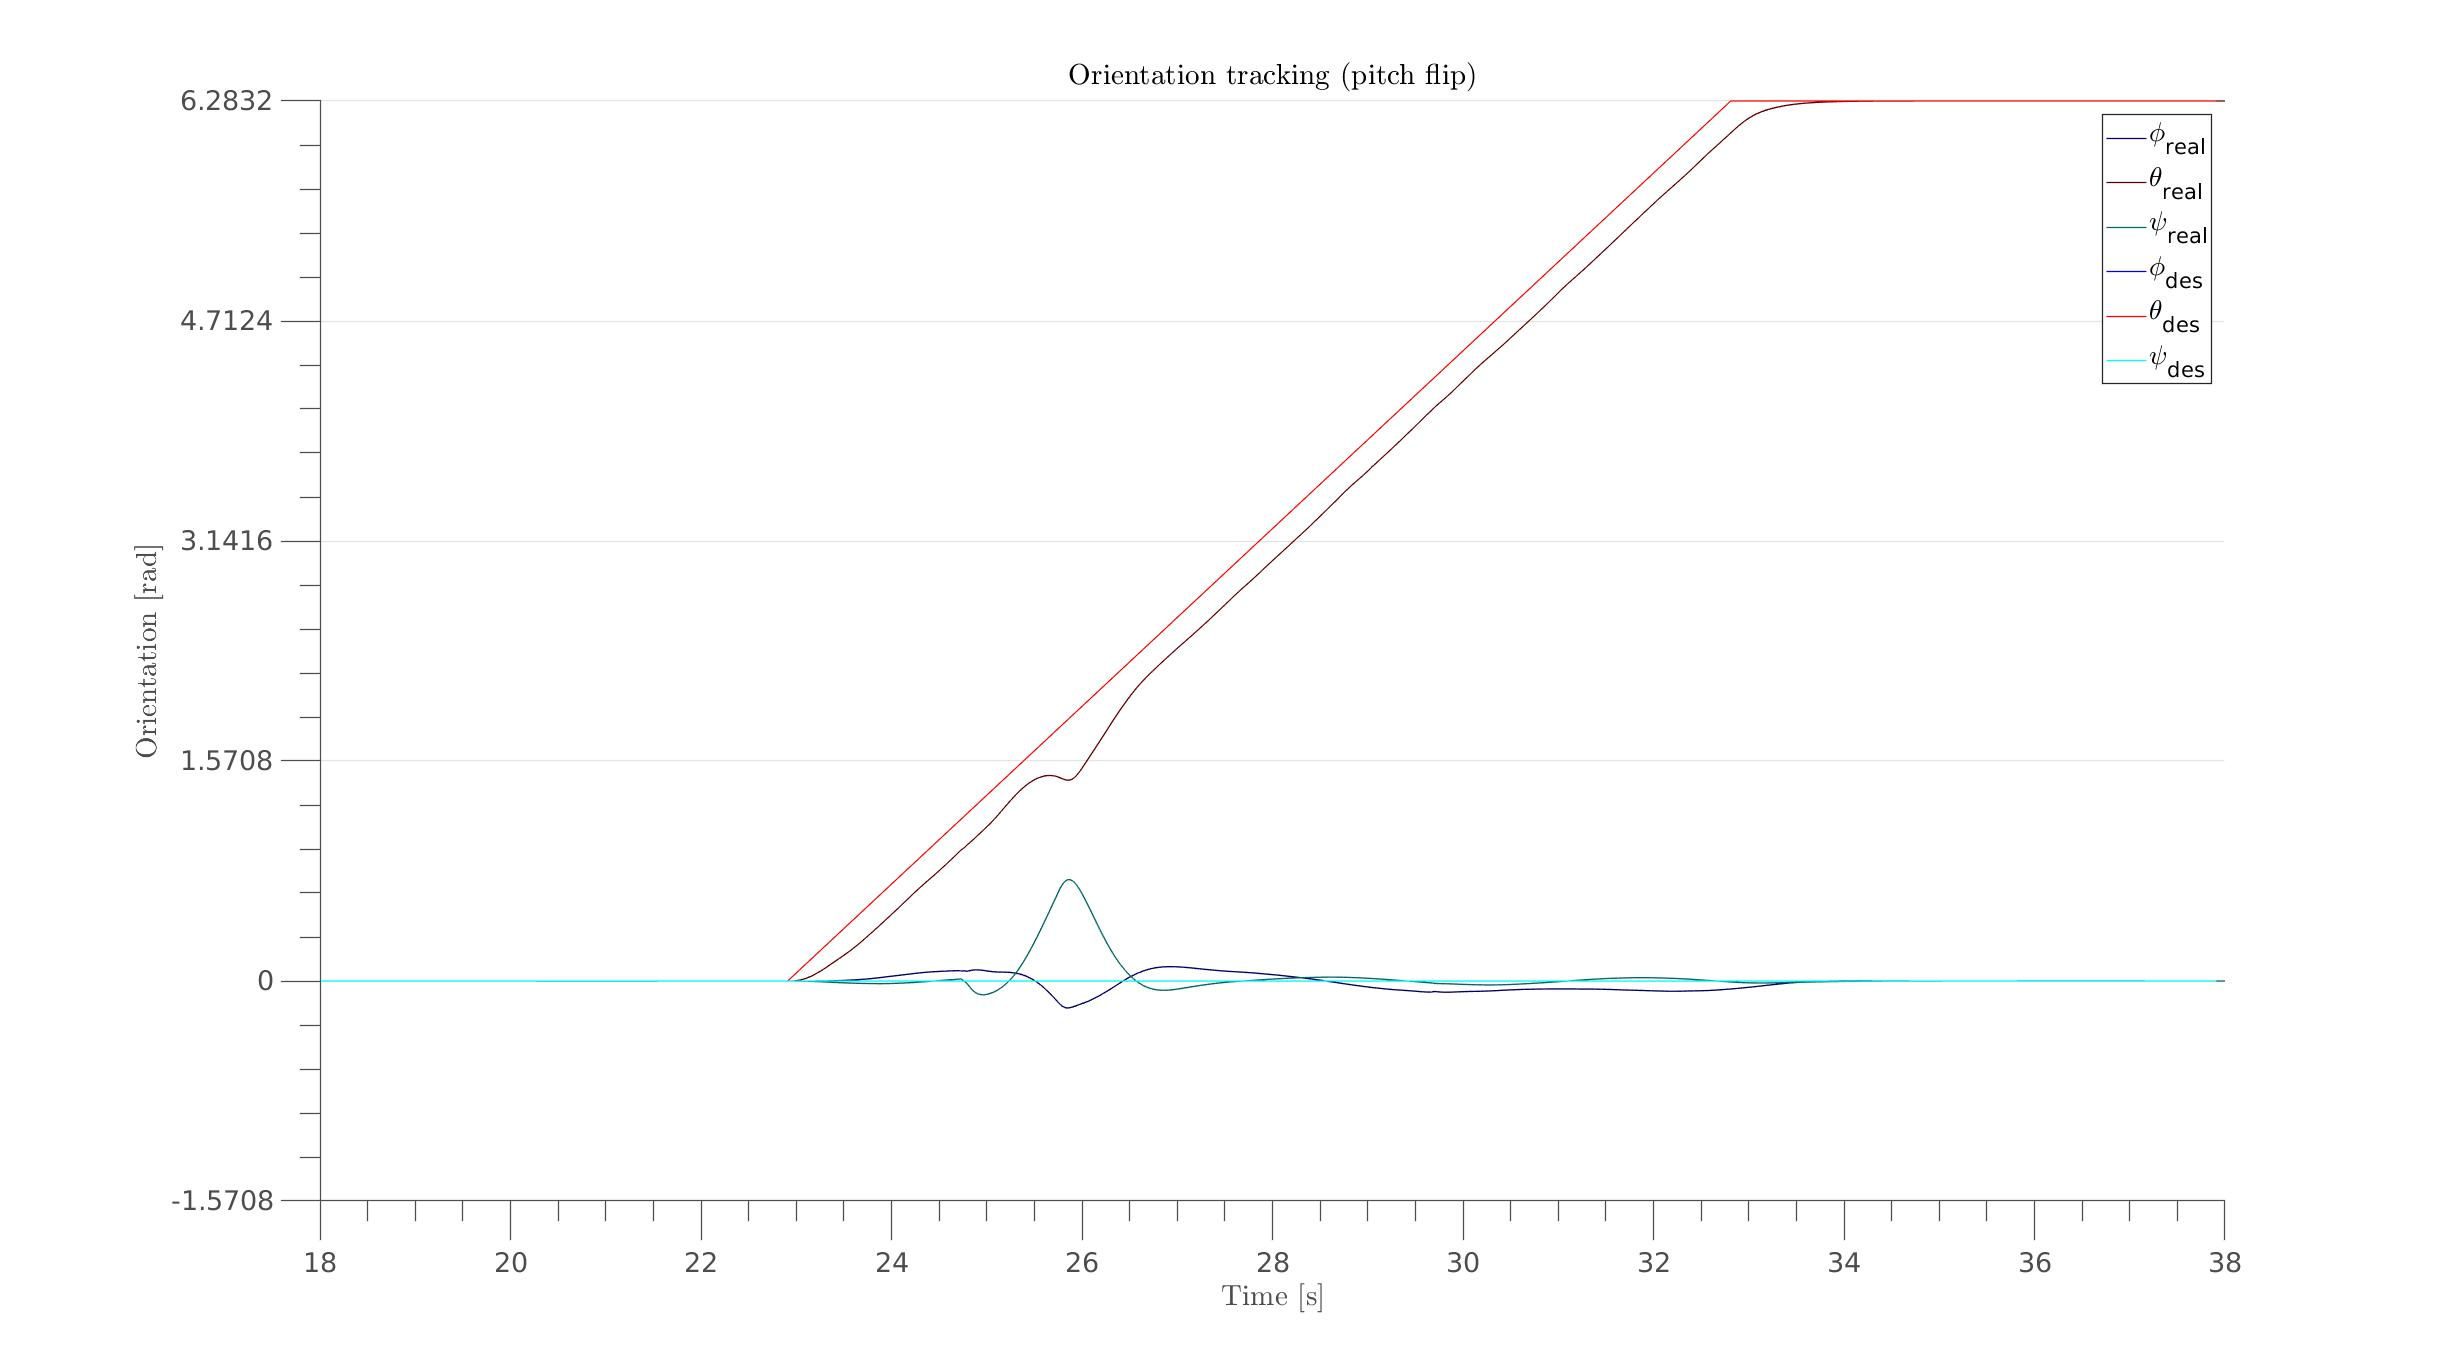
\includegraphics[width=1.0\linewidth]{images/Hexa_pitch_angle.jpg}
    \caption{Pitch, roll and yaw angle tracking for the optimal hexa-copter performing a full pitch flip.}
    \label{fig:Hexa_angle_pitch}
  \end{center}
\end{figure}

However, the controller uses
the static allocation described in \Cref{sec:allocation} to compute the desired
tilting angles and speed for the rotors. This leads to the loss of full-actuation in
certain orientations where the static allocation matrix becomes singular.

\clearpage

\section{Hepta-copter}
\label{sec:hepta_copter_sim}

\begin{figure}[!ht]
    \begin{center}
    \begin{minipage}[t]{0.495\textwidth}
      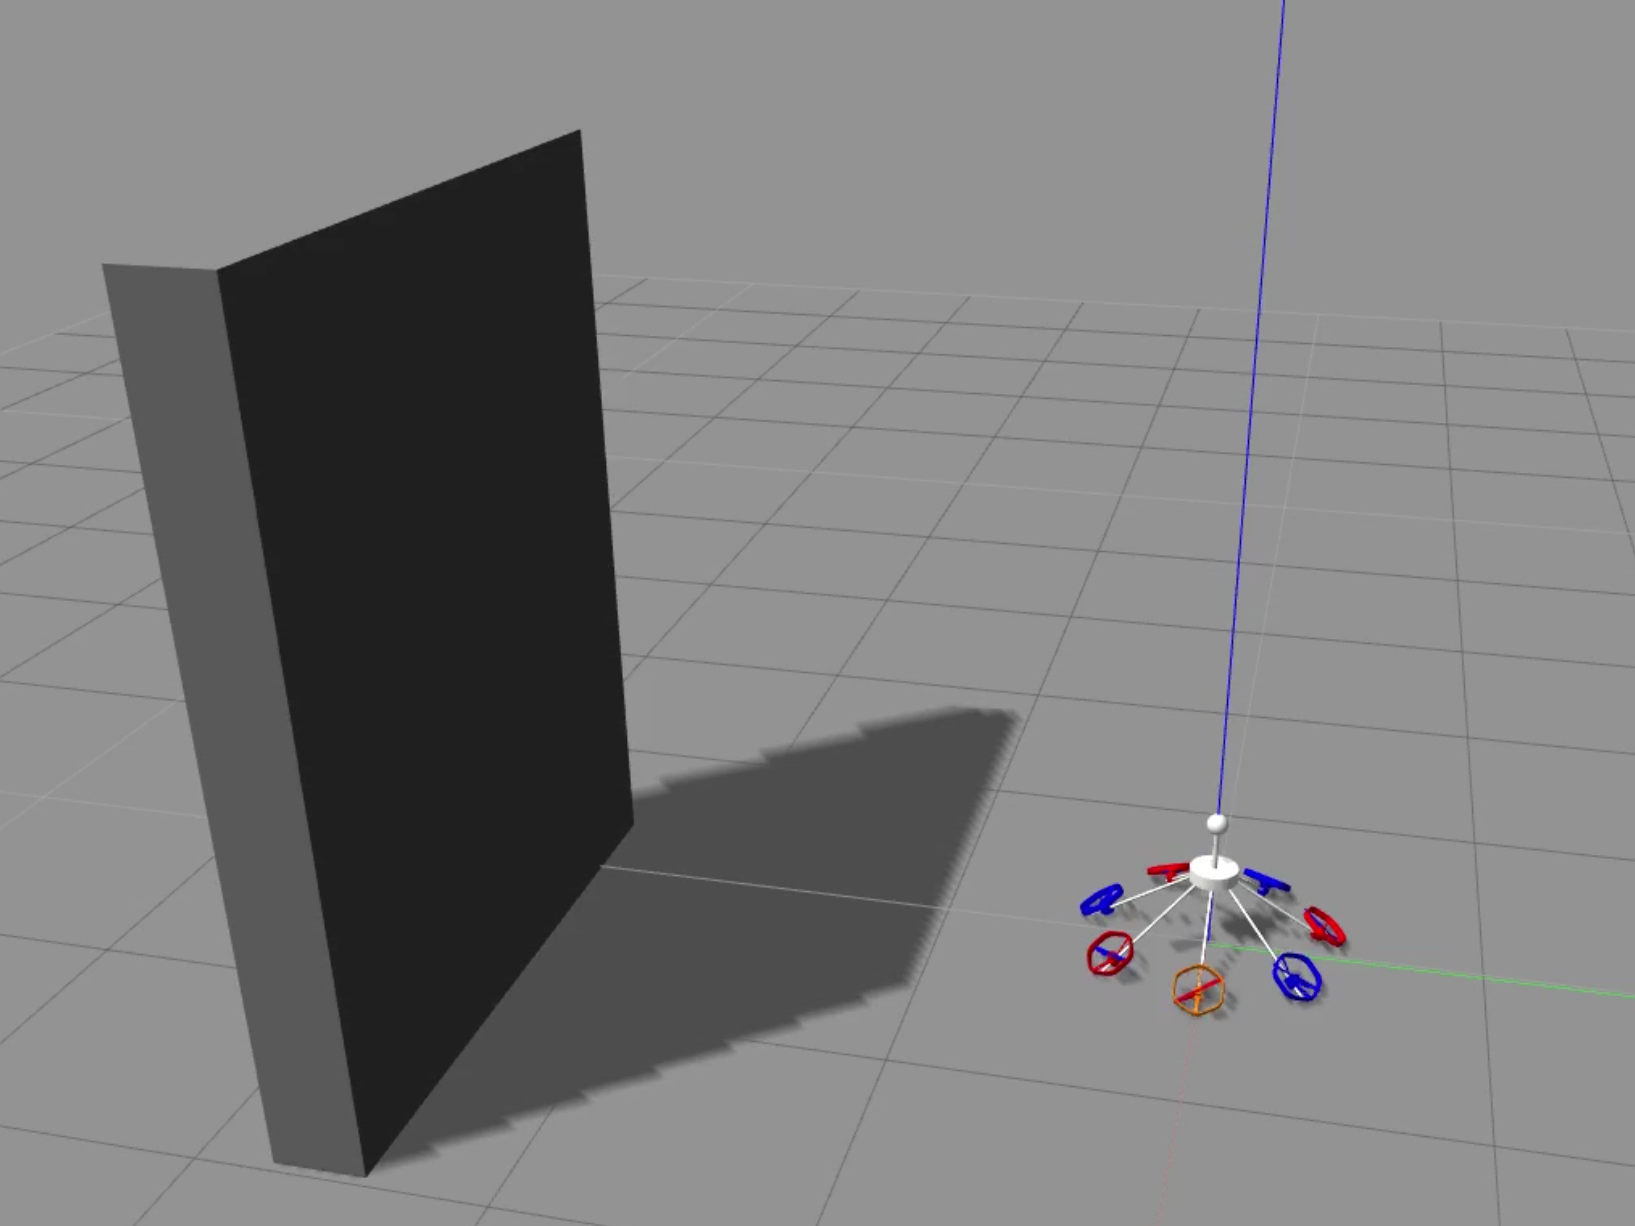
\includegraphics[width=\linewidth]{images/Selection_009.png}
    \end{minipage}
    \hfill
    \begin{minipage}[t]{0.495\textwidth}
      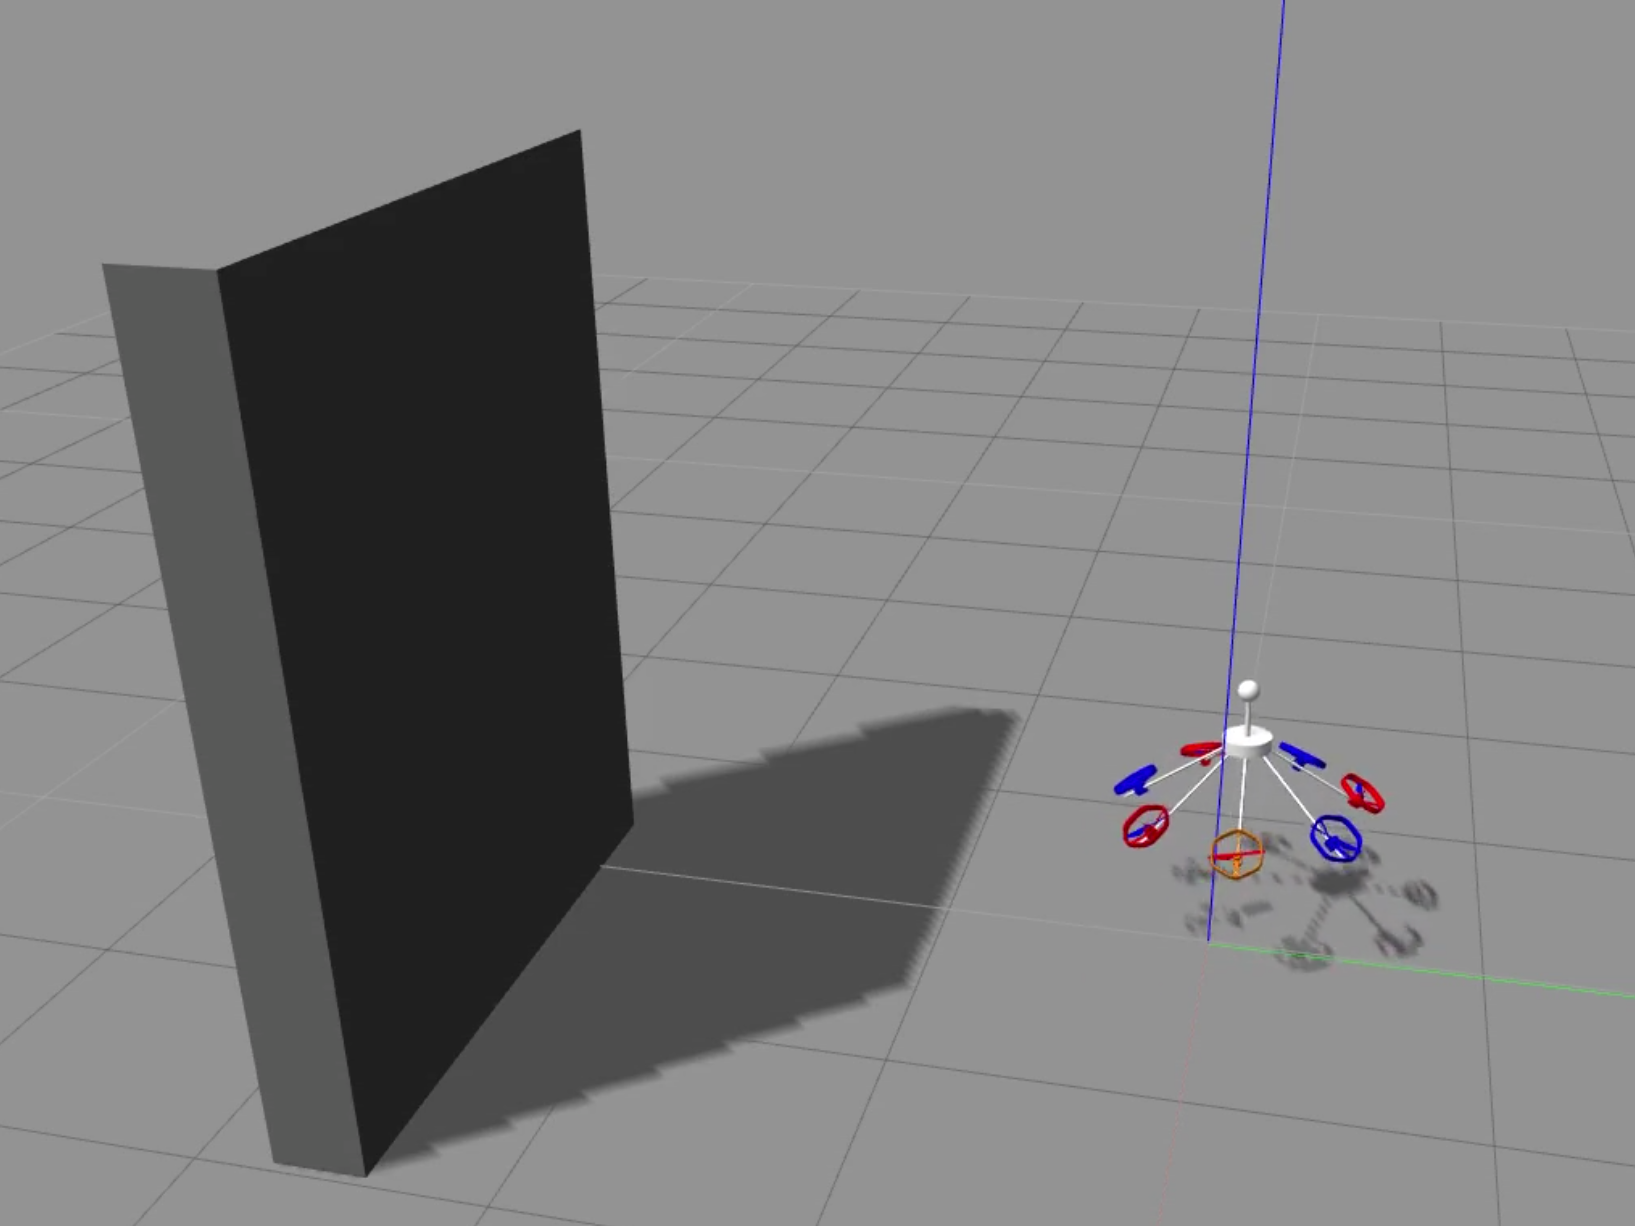
\includegraphics[width=\linewidth]{images/Selection_010.png}
    \end{minipage}
    \hfill
    \begin{minipage}[t]{0.495\textwidth}
      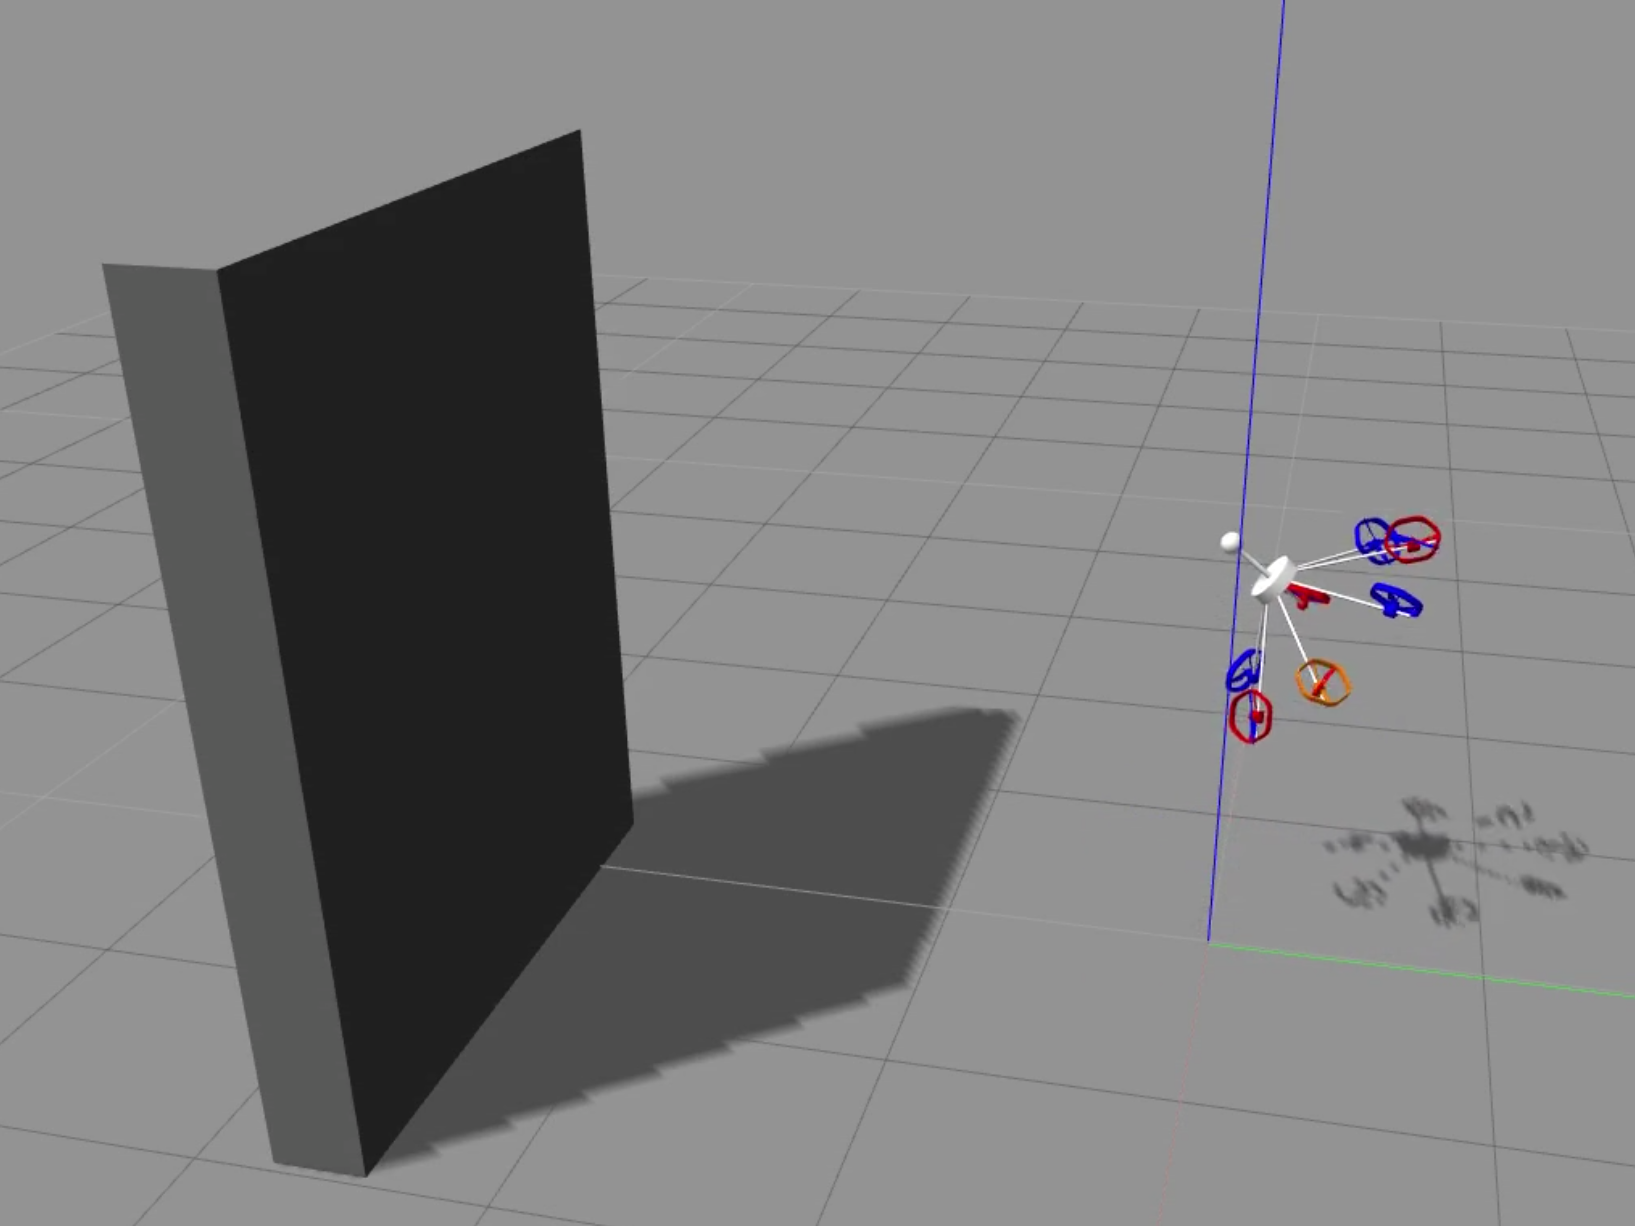
\includegraphics[width=\linewidth]{images/Selection_011.png}
    \end{minipage}
    \hfill
    \begin{minipage}[t]{0.495\textwidth}
      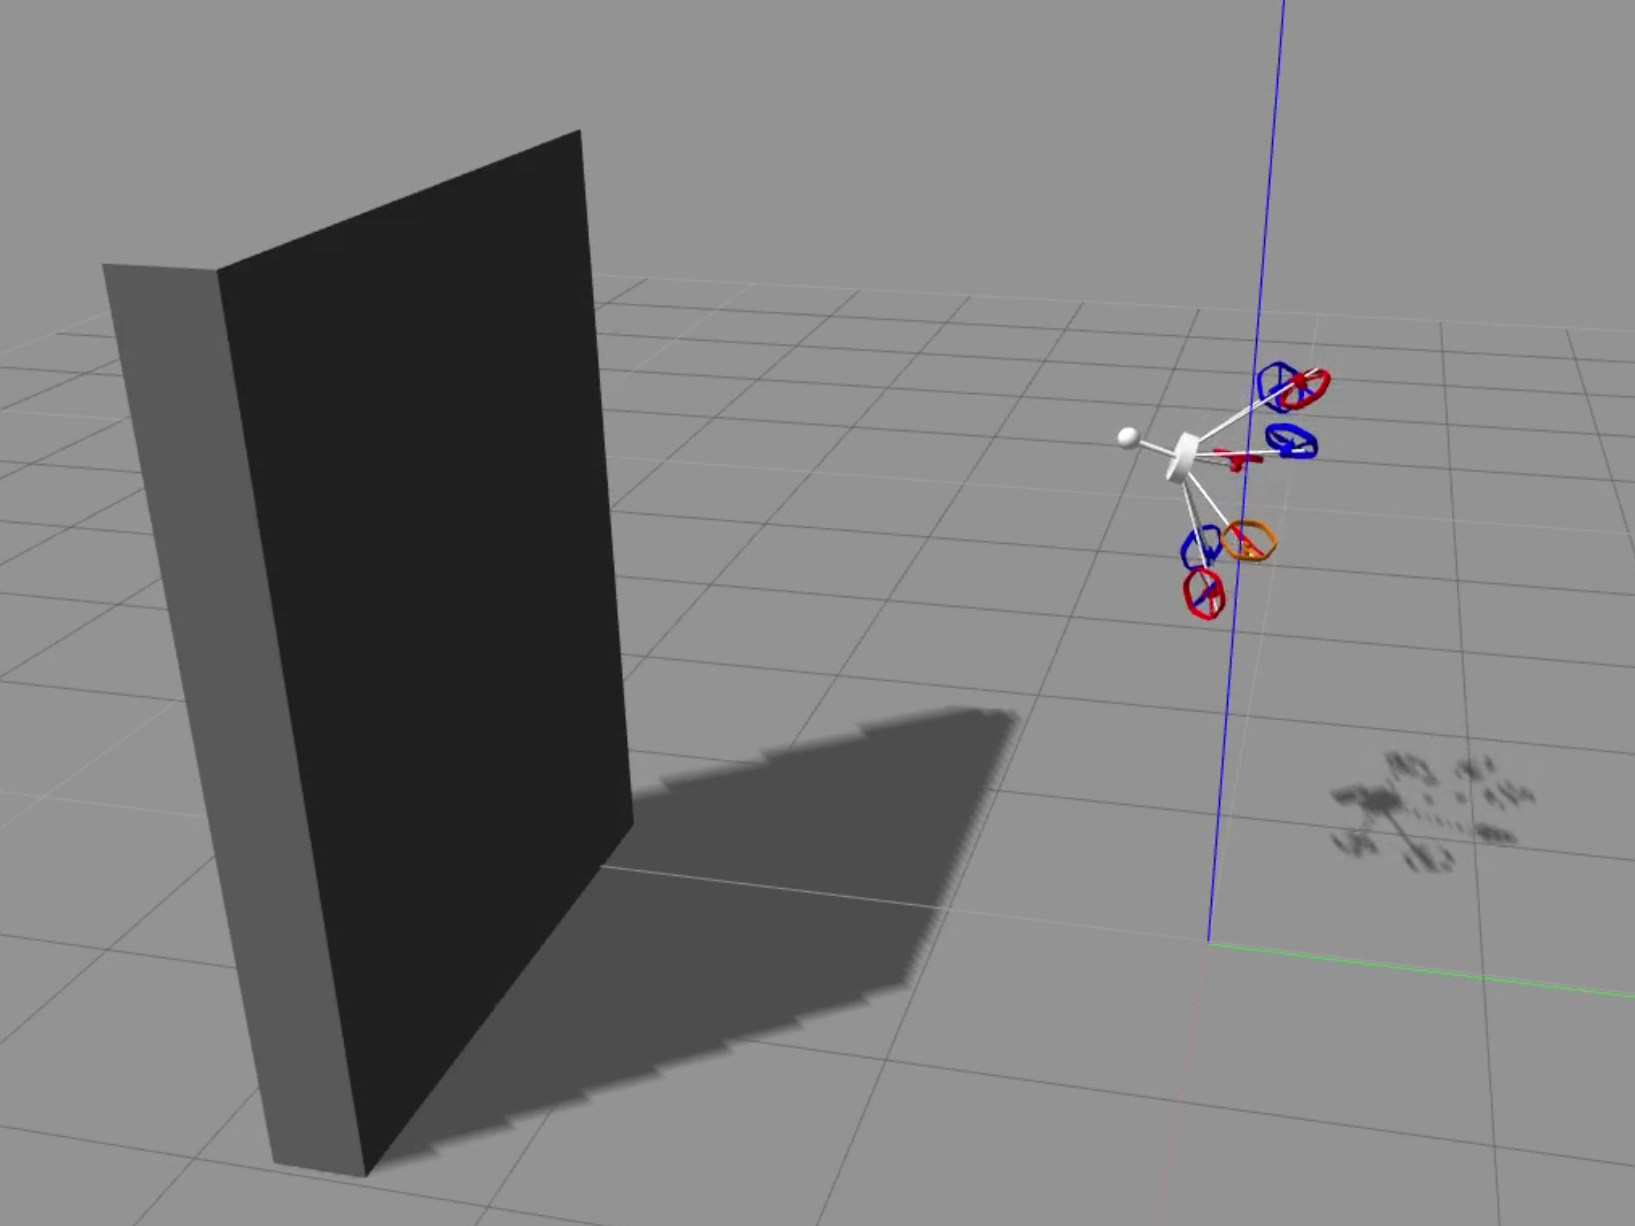
\includegraphics[width=\linewidth]{images/Selection_013.png}
    \end{minipage}
    \hfill
    \begin{minipage}[t]{0.495\textwidth}
      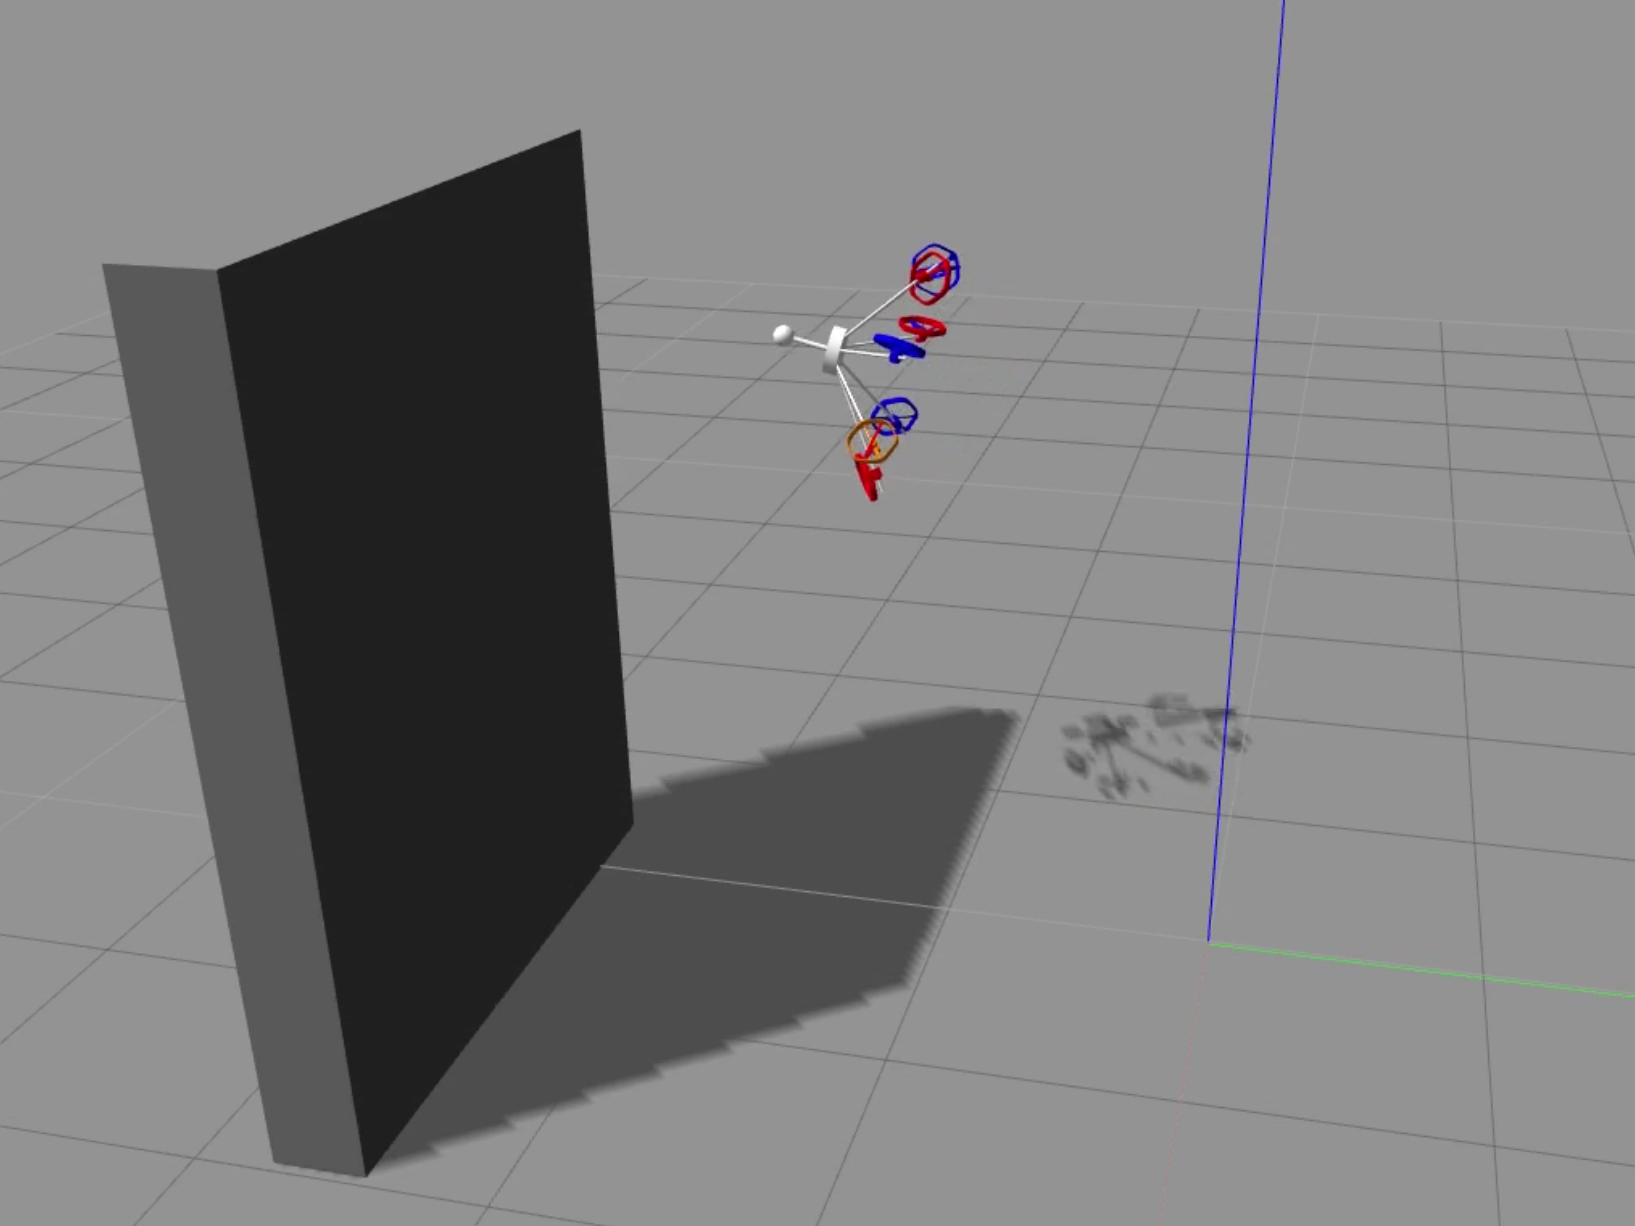
\includegraphics[width=\linewidth]{images/Selection_017.png}
    \end{minipage}
    \hfill
    \begin{minipage}[t]{0.495\textwidth}
      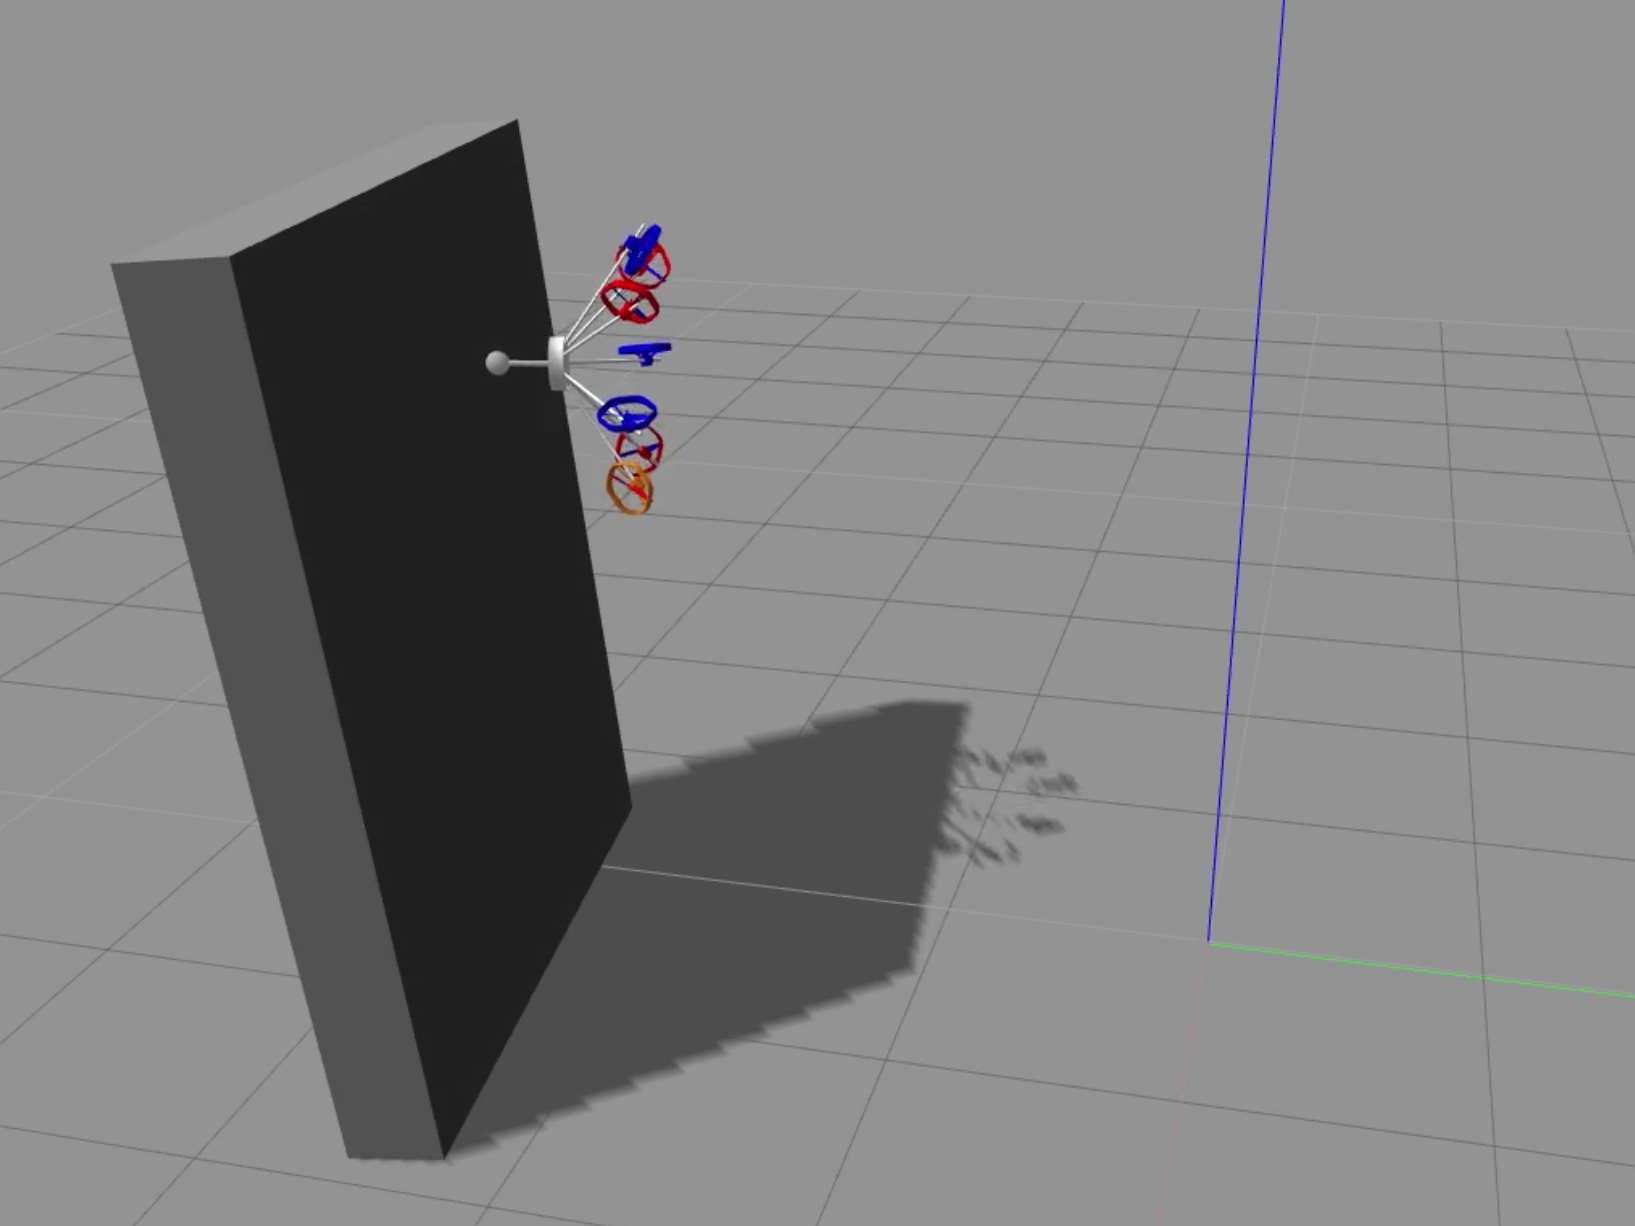
\includegraphics[width=\linewidth]{images/Selection_019.png}
    \end{minipage}
    \hfill
    \begin{minipage}[t]{0.495\textwidth}
      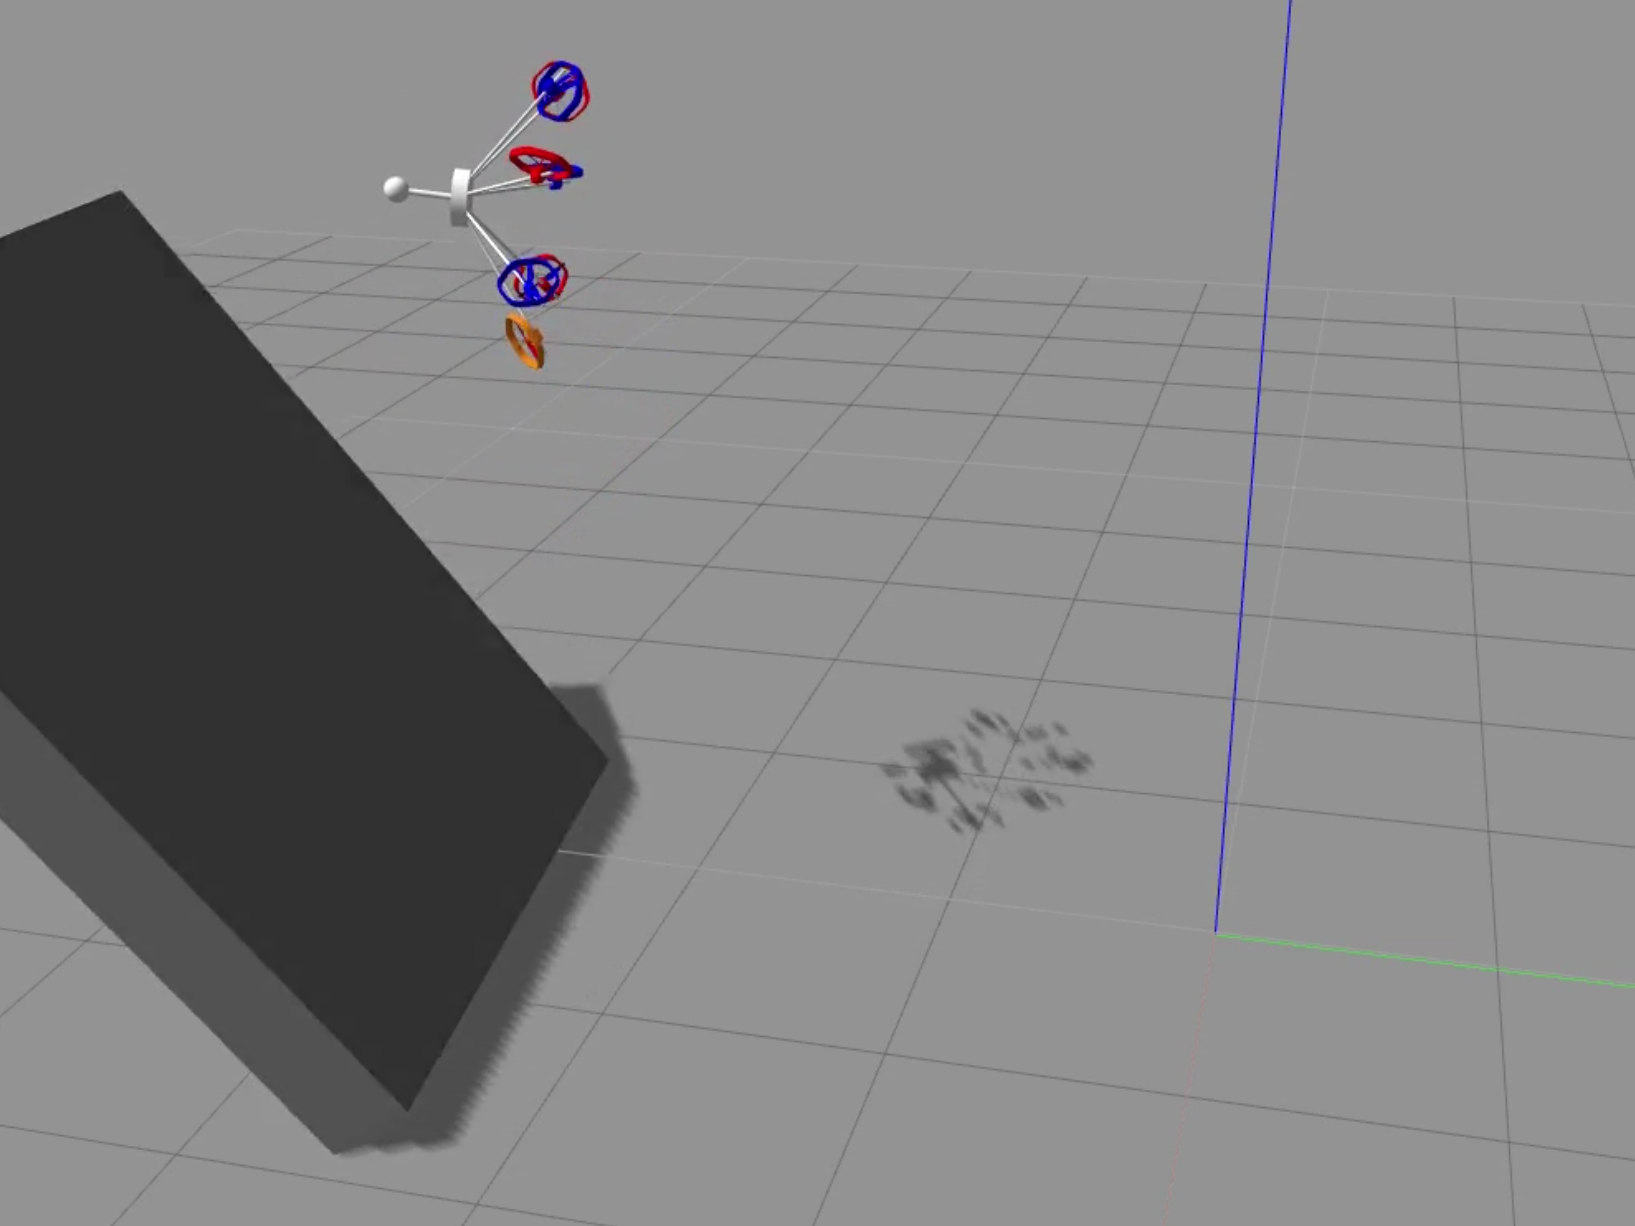
\includegraphics[width=\linewidth]{images/Selection_024.png}
    \end{minipage}
    \hfill
    \begin{minipage}[t]{0.495\textwidth}
      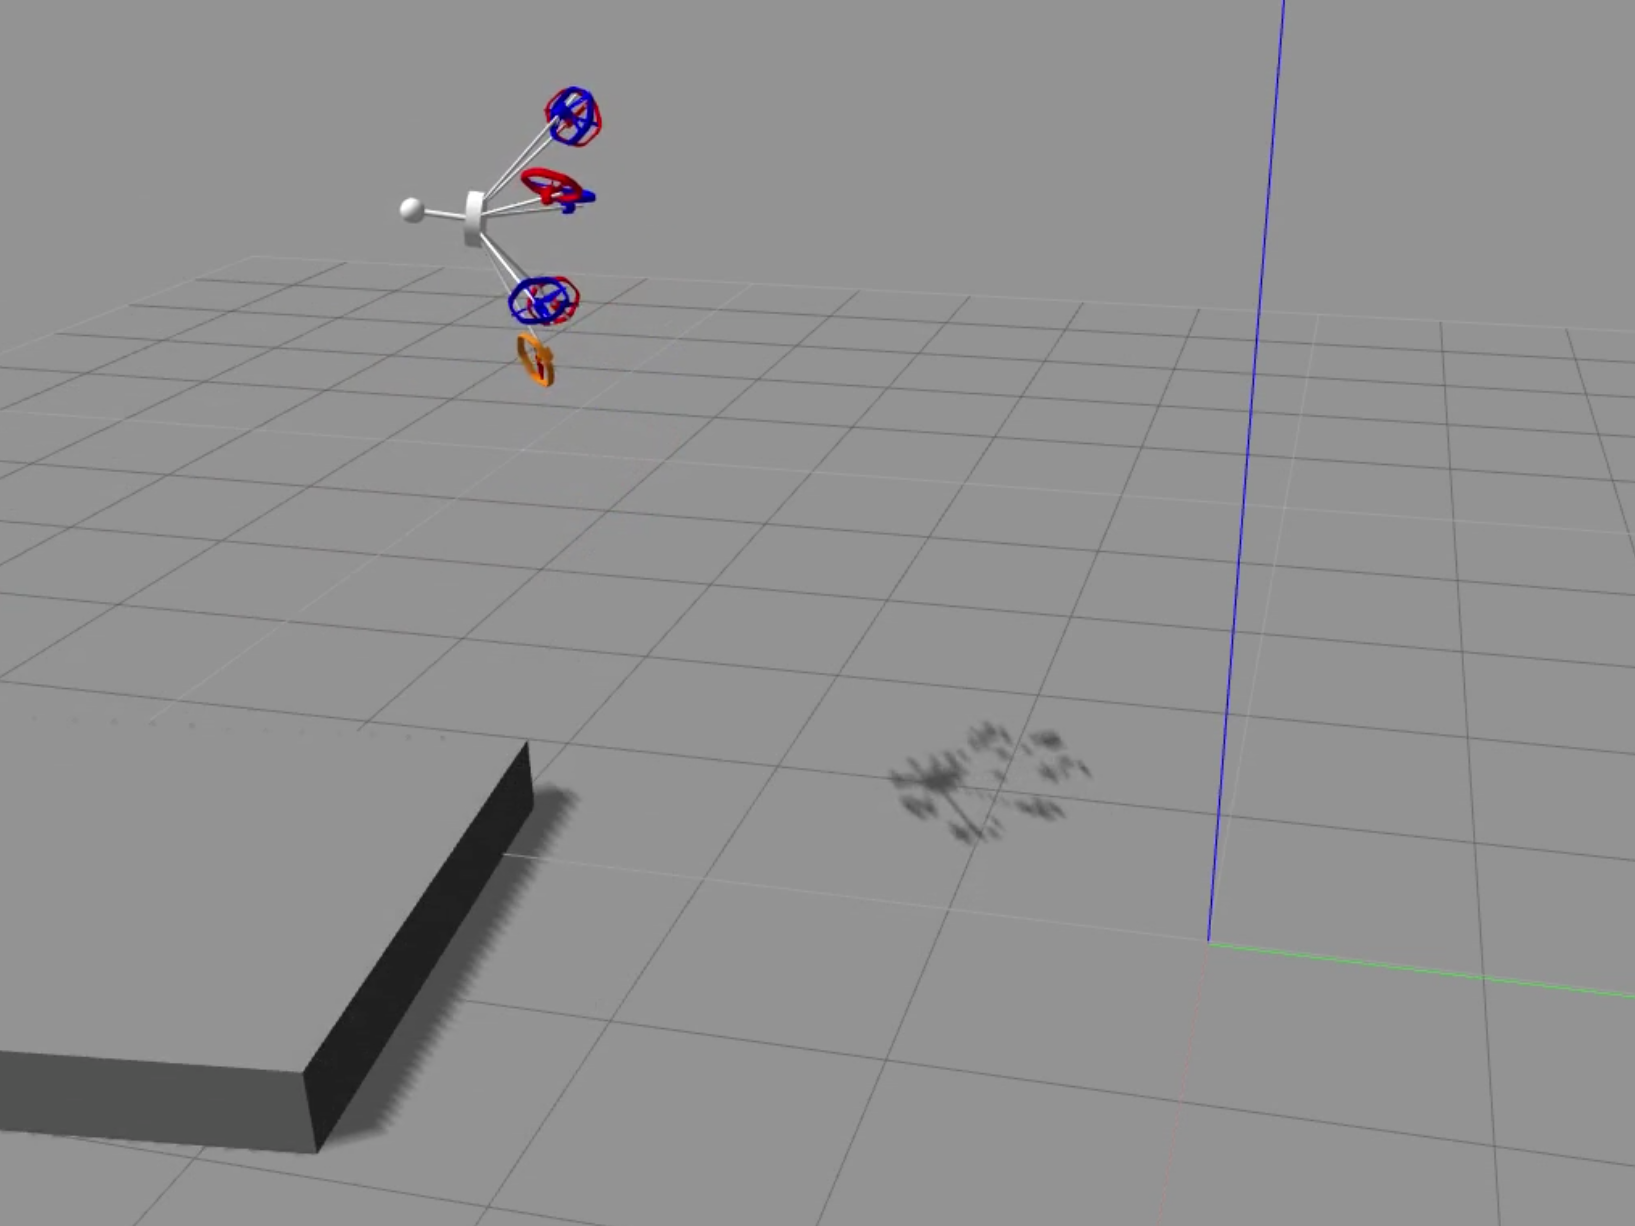
\includegraphics[width=\linewidth]{images/Selection_026.png}
    \end{minipage}
    \caption{Slideshow of an interacion between the optimal hepta-copter and a wall.}
    \label{fig:hepta_sim}
  \end{center}
\end{figure}
